\documentclass[conference,10pt]{IEEEtran}
\IEEEoverridecommandlockouts
\usepackage[T1]{fontenc}
\usepackage{graphicx,booktabs,amsmath,amssymb,xcolor,url,xspace,textcomp}
\usepackage[hidelinks]{hyperref}
\hypersetup{pdftitle={Egocentric Laundry Folding: Replaying Hand-Worn-Gripper Demonstrations on a Bimanual Robot}, pdfauthor={Jeong Hwan Lee}}
\usepackage{tikz}
\usetikzlibrary{positioning,arrows.meta,shapes,fit,backgrounds}
\newcommand{\mm}{\,mm\xspace}
\def\UrlBreaks{\do\/\do\_\do\.\do\-}\def\UrlFont{\small\ttfamily}\newcommand{\code}[1]{\path{#1}}
\DeclareMathOperator*{\argmin}{arg\,min}
\DeclareMathOperator{\clip}{clip}
\DeclareMathOperator{\sgn}{sgn}
% data-flow colours (fill F / stroke S): UMI data, human trajectory, robot-feasible, robot, calibration
\definecolor{humF}{HTML}{E3F2FD}\definecolor{humS}{HTML}{1E88E5}
\definecolor{trjF}{HTML}{E8F5E9}\definecolor{trjS}{HTML}{43A047}
\definecolor{feaF}{HTML}{FFF3E0}\definecolor{feaS}{HTML}{FB8C00}
\definecolor{robF}{HTML}{FFEBEE}\definecolor{robS}{HTML}{E53935}
\definecolor{calF}{HTML}{FFFDE7}\definecolor{calS}{HTML}{F9A825}
\definecolor{senF}{HTML}{ECEFF1}\definecolor{senS}{HTML}{546E7A}

\begin{document}
\title{Egocentric Laundry Folding:\\Replaying Hand-Worn-Gripper Demonstrations\\on a Bimanual Robot}
\author{\IEEEauthorblockN{Jeong Hwan Lee}
\IEEEauthorblockA{Technical report, version 0.1, 27 October 2026\\
Repository: \texttt{egocentric-laundry-folding}}}
\maketitle

\begin{abstract}
We want a two-arm robot to fold a T-shirt from human demonstrations recorded with hand-worn grippers, without
teleoperation, and first ask whether replaying the converted human motion makes the robot do what the human did. The
demonstrator wears two HandUMI grippers (an open-source design by BrikHMP18, not ours), each carrying three AprilTags (four since 10-23), a
wrist fisheye camera and an IMU; a fixed RGB-D camera observes the tags. A camera-to-robot calibration (0.98\,px held-out),
start markers measured in the robot base frame and a calibrated tag rig (1--4\mm static error) give each jaw-tip TCP in the
robot base frame without per-take alignment, and a classifier on the wrist video gives the jaw state. The human path is
robotized by smooth warps, planned with joint-limit-aware IK and safety checks, and replayed on two reBot B601-DM arms
through an MIT-mode bridge, with every sensor and the robot log on one host clock. Single-arm replays pass 16/18 translation strokes
(median per-axis RMSE 5.5--11.6\mm) and the rotation strokes, and the right arm grasped and lifted the T-shirt from human data.
Full two-arm replays of a 33\,s demonstration (94\,s at 0.35$\times$) run reliably: the jaws close 5--19\mm above the table (human $\approx$10\mm), the robot stays
within 2--8\mm of its command at each grasp, and runs repeat within about 1\mm. The robot does not yet fold like the
human: the position error against the replayed (robotized) human path is 17\mm (right) and 30\mm (left) RMSE, open-loop replay needs the cloth where
the human's was, and wrist-camera SLAM was rejected as the trajectory source because it loses tracking exactly at grasps.
We report no success rate.
\emph{Version 0.1 (27 October 2026)} adds the training-data track (Sec.~\ref{sec:train}): 300 successful T-shirt flattening
demonstrations, a pose source that fuses fixed-camera point tracking (CoTracker3) with the tags and the IMU (held-out
hidden-marker error 16\mm left, 19\mm right, against $\approx$42\mm for tags alone), per-demo quality grades, and labels taken
\emph{before} IK, because IK$\to$FK labels move the target by p95 $\approx$58\mm at grasps. No policy result is reported yet.
\end{abstract}

% =====================================================================
\section{Introduction}\label{sec:intro}
Hand-held and hand-worn grippers in the style of UMI~\cite{chi2024umi} let a person demonstrate with an end-effector that
looks like the robot's, without a robot in the loop. Our goal is a two-arm robot that folds a T-shirt on a table from
such demonstrations, with human data as the main source rather than teleoperation.

Before training a policy on such data, we check a narrower thing: \emph{if the robot simply replays the converted human
motion, does it do what the human did?} If replay fails, a policy trained on the same labels inherits the failure. Replay
therefore serves as an end-to-end test of calibration, pose recovery, jaw labelling and conversion
(Fig.~\ref{fig:sbs}). The demonstrations are recorded with two HandUMI grippers~\cite{handumi,meza2026handumi} and
replayed on two low-cost 6-DoF arms. This report describes what was built and measured up to 21 October 2026. Its
contributions are:
\begin{itemize}
\item one world frame, the robot base frame, set once by a camera-to-robot calibration, start markers and a per-gripper tag
  rig, so that human and robot paths share it without per-take alignment (Sec.~\ref{sec:cal});
\item a conversion from the recording to a robot-feasible jaw-tip TCP path with jaw labels: tags plus depth, IMU gap
  filling, robotization by continuous warps with a per-frame quality label, and a bimanual planner with explicit safety
  checks (Sec.~\ref{sec:conv});
\item a replay and evaluation setup in which human, command and robot are on one clock and filmed by the same camera, and
  the measured results, including the methods that failed (Secs.~\ref{sec:setup}--\ref{sec:res}).
\end{itemize}

\textbf{Roadmap.} Section~\ref{sec:related} reviews related work and Sec.~\ref{sec:overview} gives an overview of the data flow
from the UMI recording (D0) to robot motion (D7). Section~\ref{sec:hw} describes the hardware, Sec.~\ref{sec:cal} the
one-time calibration that defines the shared world frame, and Sec.~\ref{sec:conv} each transformation of the chain.
Sections~\ref{sec:setup} and~\ref{sec:res} give the experimental setup and results, and
Secs.~\ref{sec:lessons}--\ref{sec:next} the lessons, limitations and next steps. Appendix~\ref{app:run} lists the
commands in data-flow order and Appendix~\ref{app:repo} the repository layout.

\textbf{Changes since v0 (21 October).} Version 0 described the \emph{replay track}: one demonstration converted and
replayed open loop. Between 22 and 27 October the goal moved to \emph{policy training}, and the pose source, the jaw
labels, the camera calibration, the training labels and the execution path were rebuilt for it. Section~\ref{sec:train} is
new and describes that track. Sections~\ref{sec:overview}--\ref{sec:res} are kept as they were, because they still
describe the replay track and its measurements; where a part of them is no longer used for training data, a boxed
\emph{v0.1 status} note says so. Table~\ref{tab:status} lists what is used now and what was replaced.

\begin{table*}[t]
\caption{What is used now (v0.1) and what it replaced}\label{tab:status}
\centering\small
\begin{tabular}{@{}p{0.12\textwidth}p{0.28\textwidth}p{0.25\textwidth}p{0.06\textwidth}p{0.19\textwidth}@{}}
\toprule
part & used now (training data) & replaced / dropped & since & why \\
\midrule
Pose source & CoTracker3 points on the fixed camera + depth + rigid gripper model, fused with tag anchors, a constant bias
and IMU acceleration only inside gaps (variant \emph{Cg}, Sec.~\ref{sec:trainpose}) & tags + depth with IMU rotation and
linear position fill (Sec.~\ref{sec:gaps}); kept for the replay track & 10-24 & tags alone are hidden at grasps; held-out
error 42$\to$16--19\mm \\
SLAM & not used & MASt3R-SLAM gap filler; ORB-SLAM3; stereo VIO. Code moved to \code{legacy/} on 10-27 & 10-23 & breaks
at grasps; scale unobservable (Sec.~\ref{sec:slam}) \\
Rotation & Mahony AHRS with rest-period gyro bias, yaw anchored at the first $\ge$2-tag frame & gyro anchored to tags with
a median still-sample bias & 10-23 & the old bias check missed a 3.8$^\circ$/s bias (5--10$^\circ$ error) \\
Arm assignment & by the gripper's side of the table ($y$ in the robot base) & by rig label & 10-22 & rig labels swapped
against the wrist cameras \\
Jaw state & ResNet-18 classifier v003 + YOLO-pose jaw tips $\to$ continuous aperture $g$ & binary ResNet-18 only;
red-tape detector (10-20) & 10-22 & 100\%/98\% (left/right) on hand labels vs 77/98\% \\
Camera $\leftrightarrow$ robot & re-solved after every camera move from the fixed tags 400/401 + table plane
(\code{robot_cam_v002}--\code{v005}); camera raised 96$\to$105$\to$113\,cm & 32-pose wrist-marker solve
(Sec.~\ref{sec:camrobot}) & 10-25 & hands left the view at 96\,cm; no robot motion needed \\
Training label & \textbf{A}: Cartesian target before IK (fusion + reBot gripper axes + 0.25\,s smoothing + table
clearance), stored absolute, learned relative & \textbf{B}: IK$\to$FK of the robotized path; kept for QA only & 10-26 & IK
choices bend the target at grasps (Sec.~\ref{sec:trainlabels}) \\
Episode window & idle trim at 10\,cm/s (0.3\,s margin) + edge-gap trim; GOLD only for fine-tuning & full protocol window
& 10-26/27 & still frames would be learned as actions \\
Execution & receding horizon: FK $\to$ compose relative chunk $\to$ limiter $\to$ Pink IK $\to$ safety, 4 of 32 steps per
cycle (Sec.~\ref{sec:deploy}) & open-loop joint-plan replay (Sec.~\ref{sec:replay}); kept for replay tests & 10-26 & a
policy needs closed loop \\
Compute & rented RTX 5090 pods for CoTracker, jaw classifier and the 3-D solve; laptop for the rest & company GPU nodes
(Ray) & 10-26 & nodes busy \\
\bottomrule
\end{tabular}
\end{table*}

\begin{figure*}[!t]
\centering
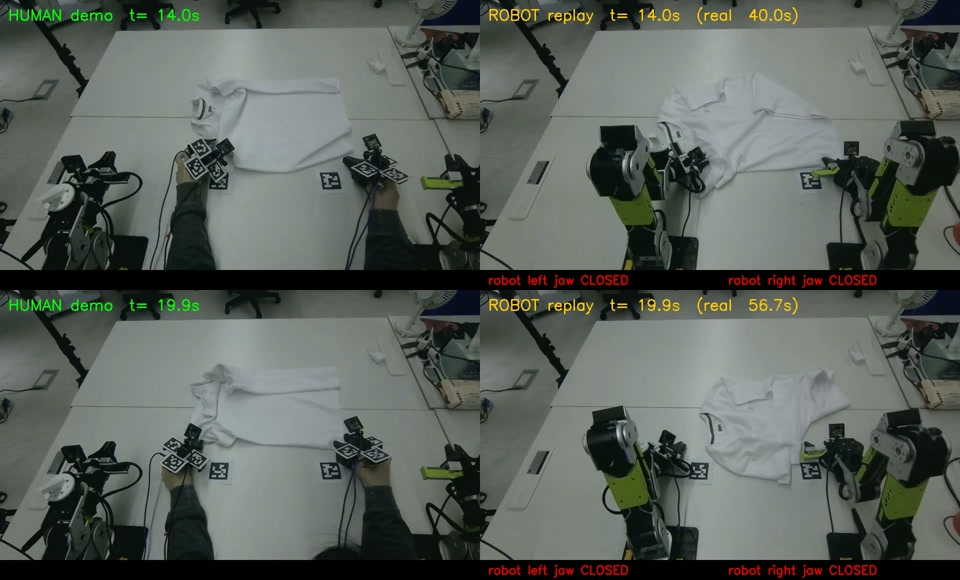
\includegraphics[width=0.92\textwidth]{figures/fig_sidebyside.jpg}
\caption{Human demonstration (left) and robot replay of the converted trajectory (right), filmed by the same fixed Orbbec
camera and aligned on one clock (take \texttt{20261021\_171057}, demo~2; run \texttt{bi\_20261021\_200335}; robot at
0.35$\times$). Rows: robot time 40\,s and 57\,s (human time 14\,s and 20\,s); the bars show the robot jaw commands. The
jaws hold the shirt edge and drag it. Full videos: \texttt{media/}.}
\label{fig:sbs}
\end{figure*}

% =====================================================================
\section{Related Work}\label{sec:related}
\subsection{Demonstration interfaces and human data}
\textbf{Hand-held and hand-worn grippers.} UMI~\cite{chi2024umi} records demonstrations with a hand-held parallel-jaw
gripper carrying a wrist fisheye camera; the end-effector pose comes from a monocular-inertial SLAM system based on
ORB-SLAM3~\cite{campos2021orbslam3}, the finger width from fiducial markers, and the trajectories are filtered by the
kinematics of the target robot. UMI also matches sensor and actuation latencies at inference and uses a relative-trajectory
action representation. HandUMI~\cite{handumi,meza2026handumi}, designed and published by BrikHMP18 and co-authors, is an
open-source hand-worn variant of UMI for robot-free bimanual data capture with swappable parallel-jaw tips; we use a build
copy of it (Sec.~\ref{sec:hw}). DexUMI~\cite{xu2025dexumi} uses the human hand with a wearable exoskeleton as the interface
for dexterous robot hands and closes the visual gap by inpainting the robot hand into the video. Our work keeps the
UMI-style gripper but replaces wrist-camera SLAM by absolute fiducial tracking from a fixed RGB-D camera, and it tests the
data by open-loop replay on the target robot before any policy training. UMI's kinematic filtering removes infeasible
trajectories; we instead warp the human path into a feasible one and store how far each frame was moved
(Sec.~\ref{sec:robotize}).

\textbf{Human and egocentric video.} EgoMimic~\cite{kareer2025egomimic} trains a single policy on egocentric human video
with 3D hand tracking together with robot demonstrations. Our long-term aim is similar (human data as the main source),
but this report covers only the step that turns hand-worn-gripper recordings into robot-frame end-effector and jaw labels
and checks them by replay.

\subsection{Robots and cloth}
\textbf{Low-cost bimanual robots.} ALOHA~\cite{zhao2023aloha} showed fine-grained bimanual manipulation with low-cost arms
and teleoperated demonstrations. We use two low-cost reBot B601-DM arms but record without teleoperation. The robot bridge
runs on a reBot plugin for LeRobot~\cite{cadene2024lerobot}.

\textbf{Cloth manipulation.} Garment folding and unfolding have been learned with dedicated primitives, e.g.\ bimanual
folding in SpeedFolding~\cite{avigal2022speedfolding} and dynamic flinging in FlingBot~\cite{ha2021flingbot}. We do not
propose a cloth method; the cloth enters our results only as the object the replayed grasps must reach.

\subsection{Pose estimation, calibration and kinematics}
\textbf{Fiducial markers.} We use AprilTag~\cite{olson2011apriltag,wang2016apriltag2} tag36h11 markers detected with
OpenCV~\cite{bradski2000opencv}. A single square tag is solved with IPPE~\cite{collins2014ippe}, which returns the two
candidate poses of a planar target; when several tags of one rig are visible, all corners are solved jointly with
SQPnP~\cite{terzakis2020sqpnp} followed by Levenberg--Marquardt refinement.

\textbf{Visual and visual-inertial SLAM.} To fill the tag-hidden grasp phases we tested
MASt3R-SLAM~\cite{murai2025mast3rslam}, a dense monocular SLAM system built on the MASt3R~\cite{leroy2024mast3r} and
DUSt3R~\cite{wang2024dust3r} two-view reconstruction priors; ORB-SLAM3~\cite{campos2021orbslam3} in monocular-inertial mode;
and, with an earlier stereo camera, Basalt~\cite{usenko2020basalt}, OpenVINS~\cite{geneva2020openvins} and
AirSLAM~\cite{xu2025airslam}. Section~\ref{sec:slam} reports why none of them became the trajectory source.

\textbf{Calibration and kinematics.} Camera--IMU calibration of the earlier pipeline used Kalibr~\cite{furgale2013kalibr}.
The camera-to-robot transform is initialised with the robot-world/hand-eye solution of Shah~\cite{shah2013robotworld} (as
implemented in OpenCV) and refined by our own least squares. Inverse kinematics uses Pink~\cite{pink} on top of
Pinocchio~\cite{carpentier2019pinocchio}. The jaw classifier is a ResNet-18~\cite{he2016resnet} pretrained on
ImageNet~\cite{deng2009imagenet}.

% =====================================================================
\section{System Overview}\label{sec:overview}
\begin{figure*}[!t]
\centering
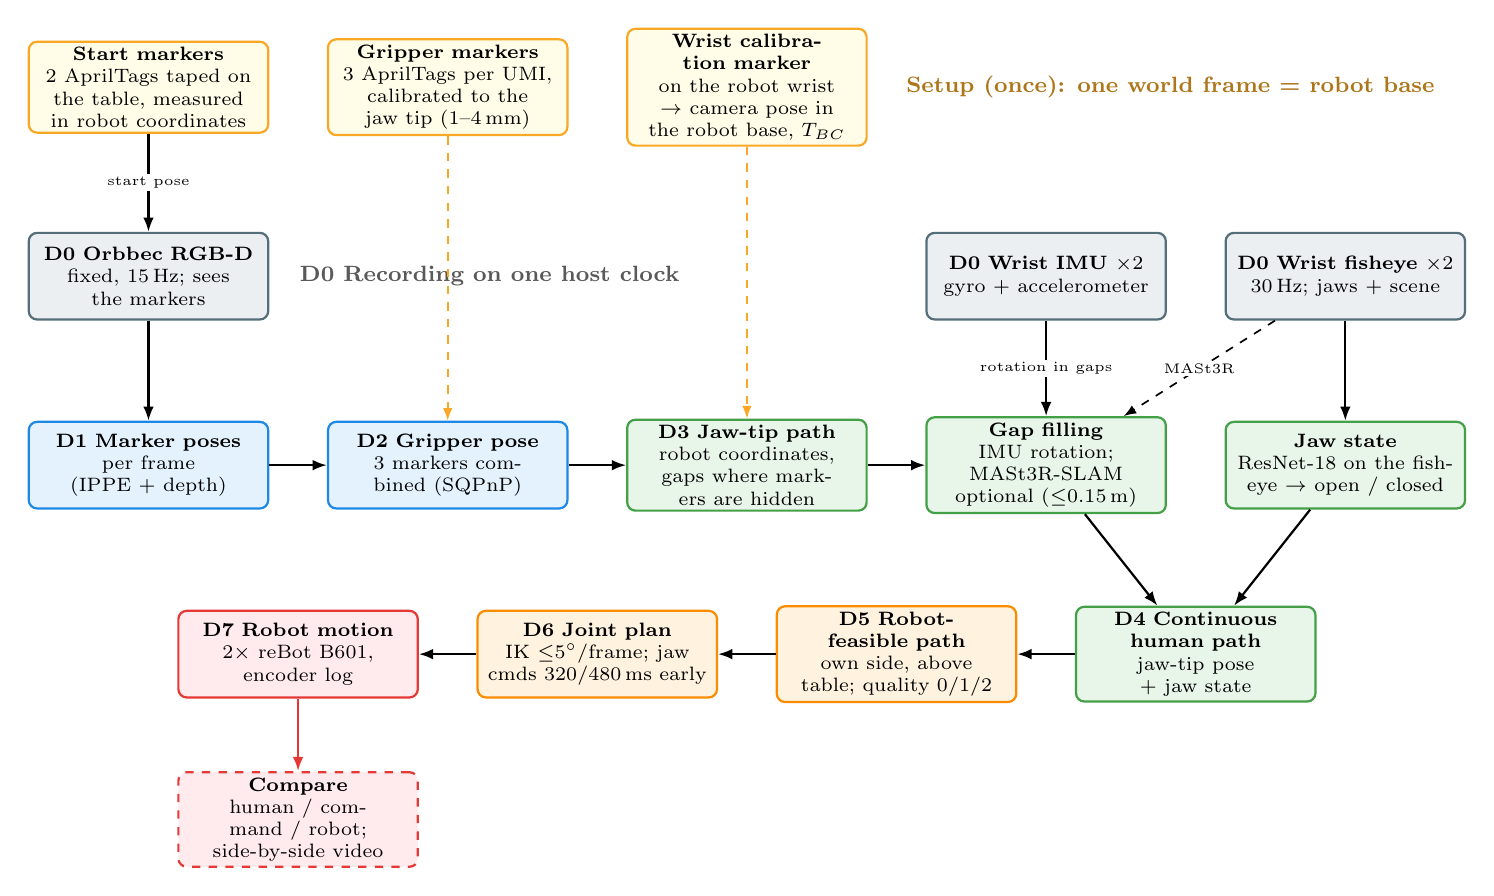
\begin{tikzpicture}[
  font=\scriptsize,
  arr/.style={-{Latex[length=1.8mm]},thick},
  darr/.style={-{Latex[length=1.6mm]},dashed,semithick},
  box/.style={draw=#1S, fill=#1F, rounded corners=3pt, line width=0.8pt, text width=29mm, minimum height=11mm,
    align=center, inner sep=2pt},
  elab/.style={font=\tiny, align=center, fill=white, inner sep=1pt}]
% ---- row 1: one-time setup with AprilTag markers
\node[box=cal] (s2) at (0,0)    {\textbf{Start markers}\\2 AprilTags taped on the table, measured in robot coordinates};
\node[box=cal] (s3) at (3.8,0)  {\textbf{Gripper markers}\\3 AprilTags per UMI, calibrated to the jaw tip (1--4\,mm)};
\node[box=cal] (s1) at (7.6,0)  {\textbf{Wrist calibration marker}\\on the robot wrist $\to$ camera pose in the robot base, $T_{BC}$};
\node[font=\footnotesize\bfseries, text=calS!70!black, anchor=west] at (9.5,0) {Setup (once): one world frame = robot base};
% ---- row 2: D0 sensors
\node[box=sen] (orb) at (0,-2.4)    {\textbf{D0 Orbbec RGB-D}\\fixed, 15\,Hz; sees the markers};
\node[box=sen] (imu) at (11.4,-2.4) {\textbf{D0 Wrist IMU} $\times$2\\gyro + accelerometer};
\node[box=sen] (fis) at (15.2,-2.4) {\textbf{D0 Wrist fisheye} $\times$2\\30\,Hz; jaws + scene};
\node[font=\footnotesize\bfseries, text=gray!70!black, anchor=west] at (1.8,-2.4) {D0 Recording on one host clock};
% ---- row 3: human data -> robot coordinates
\node[box=hum] (d1) at (0,-4.8)    {\textbf{D1 Marker poses}\\per frame (IPPE + depth)};
\node[box=hum] (d2) at (3.8,-4.8)  {\textbf{D2 Gripper pose}\\3 markers combined (SQPnP)};
\node[box=trj] (d3) at (7.6,-4.8)  {\textbf{D3 Jaw-tip path}\\robot coordinates, gaps where markers are hidden};
\node[box=trj] (gf) at (11.4,-4.8) {\textbf{Gap filling}\\IMU rotation; MASt3R-SLAM optional ($\le$0.15\,m)};
\node[box=trj] (jw) at (15.2,-4.8) {\textbf{Jaw state}\\ResNet-18 on the fisheye $\to$ open / closed};
% ---- row 4: robot side (right to left)
\node[box=trj] (d4) at (13.3,-7.2) {\textbf{D4 Continuous human path}\\jaw-tip pose + jaw state};
\node[box=fea] (d5) at (9.5,-7.2)  {\textbf{D5 Robot-feasible path}\\own side, above table; quality 0/1/2};
\node[box=fea] (d6) at (5.7,-7.2)  {\textbf{D6 Joint plan}\\IK $\le$5$^\circ$/frame; jaw cmds 320/480\,ms early};
\node[box=rob] (d7) at (1.9,-7.2)  {\textbf{D7 Robot motion}\\2$\times$ reBot B601, encoder log};
\node[box=rob, dashed] (cmp) at (1.9,-9.3) {\textbf{Compare}\\human / command / robot; side-by-side video};
% ---- edges
\draw[arr] (s2) -- node[elab]{start pose} (orb);
\draw[arr] (orb) -- (d1);
\draw[arr] (d1) -- (d2);
\draw[arr] (d2) -- (d3);
\draw[arr] (d3) -- (gf);
\draw[darr,draw=calS] (s3) -- (d2);
\draw[darr,draw=calS] (s1.south) .. controls (7.6,-2.4) .. (d3.north);
\draw[arr] (imu) -- node[elab]{rotation in gaps} (gf);
\draw[darr] (fis) -- node[elab]{MASt3R} (gf);
\draw[arr] (fis) -- (jw);
\draw[arr] (gf) -- (d4);
\draw[arr] (jw) -- (d4);
\draw[arr] (d4) -- (d5);
\draw[arr] (d5) -- (d6);
\draw[arr] (d6) -- (d7);
\draw[arr,draw=robS] (d7) -- (cmp);
\end{tikzpicture}
\caption{Data flow from the UMI recording to robot motion. Yellow: one-time setup with AprilTag markers that puts human and
robot in one world frame (the robot base). Grey: the three sensors of the recording D0. Blue: marker and gripper poses in
the camera frame. Green: the human jaw-tip path in robot coordinates, completed by IMU gap filling (MASt3R-SLAM optional)
and the jaw state from the wrist fisheye. Orange: robot-feasible path and joint plan. Red: robot and comparison. Dashed:
calibration inputs and the optional SLAM filler. v0.1: this is the replay track; the training-data track is in
Sec.~\ref{sec:train}.}
\label{fig:pipe}
\end{figure*}

Figure~\ref{fig:pipe} shows how a demonstration becomes robot motion as a chain of data artifacts D0--D7. Two principles
run through it: every pose lives in one world frame, the robot base frame, and every sensor and robot log is stamped by
one host clock.
\begin{itemize}
\item \emph{Setup with AprilTag markers} (yellow, once; Sec.~\ref{sec:cal}): a calibration marker on the robot wrist gives
  the camera pose in the robot base, two start markers on the table are measured in robot coordinates, and the three
  markers on each gripper are calibrated to its jaw tip. Every take starts with the grippers at the start markers.
\item \emph{Recording D0} (grey; Sec.~\ref{sec:rec}): three sensors on one clock. The fixed Orbbec RGB-D camera sees the
  markers and is the main position source; the wrist IMU supplies rotation while the markers are hidden; the wrist fisheye
  shows the jaws (jaw state) and the scene (optional MASt3R-SLAM).
\item \emph{Marker and gripper poses} (blue): per-frame marker poses D1 (Sec.~\ref{sec:tagdet}) and the gripper pose D2
  (Sec.~\ref{sec:rigpose}), in the camera frame.
\item \emph{Human path in robot coordinates} (green): the jaw-tip path D3 (Sec.~\ref{sec:tcp}); IMU gap filling, the
  optional MASt3R filler and the jaw state make it the continuous path D4 (Sec.~\ref{sec:gaps}).
\item \emph{Robot-feasible path and plan} (orange): robotization gives D5 (Sec.~\ref{sec:robotize}); IK gives the joint
  plan with jaw commands D6 (Sec.~\ref{sec:plan}), executed only if the safety checks pass (Sec.~\ref{sec:checks}).
\item \emph{Robot} (red): the bridge executes the plan and logs the robot motion D7 (Sec.~\ref{sec:replay}), which is
  compared with D4/D5 and filmed by the same camera (Sec.~\ref{sec:setup}).
\end{itemize}

% =====================================================================
\section{Hardware}\label{sec:hw}
\begin{table}[t]
\caption{Components}\label{tab:hw}
\centering\small
\begin{tabular}{@{}p{0.27\columnwidth}p{0.65\columnwidth}@{}}
\toprule
unit & model, role \\
\midrule
Hand-worn gripper $\times$2 & HandUMI~\cite{handumi} (BrikHMP18), our build; human demonstration tool \\
Wrist camera $\times$2 & fisheye, 1280$\times$720 at 30\,Hz (left measured 24\,fps in take 171057); jaw state, optional SLAM \\
Wrist IMU $\times$2 & Seeed XIAO nRF52840 Sense; gyro and accelerometer \\
RGB-D camera & Orbbec Gemini 336, colour + aligned depth at 15\,Hz, fixed $\approx$0.8\,m above the table (v0.1: raised to 1.13\,m on 10-25) \\
Robot arms $\times$2 & reBot B601-DM, 6-DoF + parallel jaw, Damiao motors on USB-CAN \\
Host & Apple-silicon laptop: recording, planning, bridge \\
GPU & v0: RTX 4090/5090 nodes for MASt3R-SLAM; v0.1: rented RTX 5090 pods for CoTracker3, the jaw classifier and the 3-D solve \\
\bottomrule
\end{tabular}
\end{table}

Table~\ref{tab:hw} lists the components.

\subsection{HandUMI and our modifications}
\begin{figure}[!t]
\centering
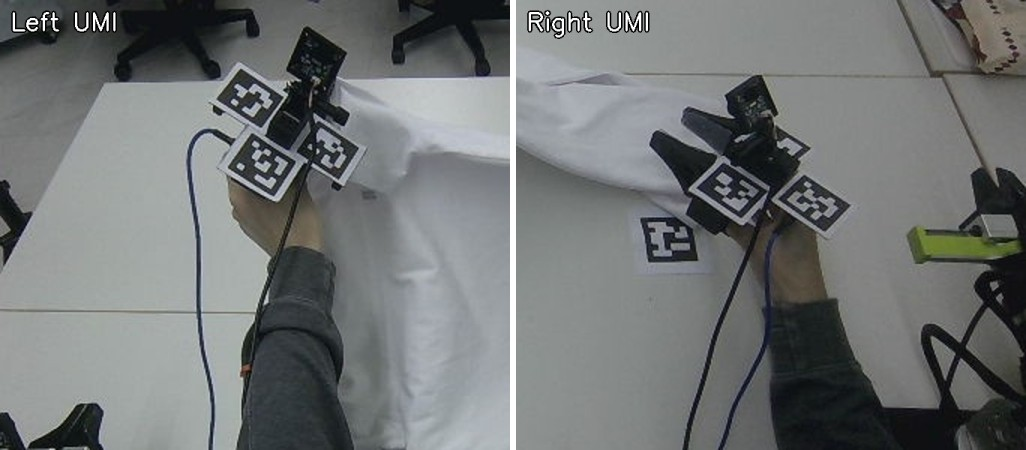
\includegraphics[width=\columnwidth]{figures/fig_umi.jpg}
\caption{The UMI hands as used now (cut from a demo recording): HandUMI with three 48\mm AprilTags per hand (left UMI on the left, IDs 210--212;
right UMI on the right, IDs 200--202), wrist fisheye and IMU; no jaw servo. Photo from before 10-23: since then a fourth, 30\mm tag sits on the back of each wrist camera (IDs 220 / 221).}
\label{fig:umi}
\end{figure}

HandUMI~\cite{handumi,meza2026handumi} is a hand-worn parallel-jaw gripper designed and published by BrikHMP18
(Apache-2.0). It is not our design. We print the upstream parts (commit \texttt{e58de33}) and changed the following
(Fig.~\ref{fig:umi}):
\begin{itemize}
\item three modified parts: a controller-support part turned into a connector with a +10\mm plate (we use no VR
  controller), a camera mount with an extra window, and a servo cover with a wider cable opening;
\item a wrist IMU instead of VR tracking (first a Teensy 4.1 with an ICM-42688-P, now a Seeed XIAO nRF52840 Sense per hand);
\item the jaw servos removed on 10-13, because the servo shafts broke and the units were heavy;
\item the red jaw tape removed on 10-20, because the colour detector fired on background objects;
\item three tag36h11 AprilTags per hand (48\mm black square, on different faces so that at least one faces the camera in
  most poses);
\item since 10-23 a fourth tag per hand: a 30\mm tag on the back of the wrist camera (ID 220 on the 210--212 UMI, 221 on
  the 200--202 UMI; rig calibration \texttt{umi\_tag\_rig\_v002}). Alone, this small planar tag has a pose flip (IPPE
  ambiguity, p90 70--130\mm TCP error), so a pose from it alone is accepted only when the IMU picks the right solution;
  frames with any of the 48\mm tags use the normal multi-tag PnP.
\end{itemize}
Both wrist fisheye cameras report the same serial number, so they are identified by USB location.

\subsection{Scene and robot arms}


The Orbbec Gemini 336 is fixed about 0.8\,m above the table (camera origin at $z=0.79$\,m in $T_{BC}$; its view is Fig.~\ref{fig:start}). Two reBot B601-DM arms are mounted
560\mm apart (tape; the URDF assumes 630\mm). Two \emph{start markers} (AprilTags with IDs 400 and 401, 60\mm) are taped on the table where the left and right
grippers are placed at the start of every take, and a \emph{wrist calibration marker} (AprilTag ID 220, 50\mm) is fixed
on the wrist-roll motor body of the robot so the camera can locate the robot. The gripper zeros drift at every power cycle and are
read before each session; the left jaw travel is limited to half.

\subsection{Robot bridge}\label{sec:bridge}
Our HTTP service drives both arms from one 100\,Hz thread with synchronised, acceleration-limited motion toward each goal
(45$^\circ$/s, 180$^\circ$/s$^2$), goal interpolation between streamed commands, and parking with torque off at rest.

\textbf{Control law.} In MIT mode each drive receives a position and velocity reference, gains, and a feed-forward torque.
The bridge uses an integral-only feed-forward law and no gravity model:
\begin{align}
\tau&=K_p\,e+K_d\,\dot e+\tau_\mathrm{ff},\quad e=q^\star-q,\\
\tau_\mathrm{ff}[k+1]&=\tau_\mathrm{ff}[k]+K_i\,e[k]\,\Delta t .
\end{align}
While the arm moves, the joint torque must follow the changing gravity load $\tau_g$. In quasi-steady motion
($\dot e\approx0$), differentiating the torque balance $\tau_g=K_p e+\tau_\mathrm{ff}$ gives $\dot\tau_g=K_p\dot e+K_i e$,
hence
\begin{equation}
e\approx\dot\tau_g/K_i,
\end{equation}
independent of $K_p$. This matched the measurements: raising $K_p$ on j2/j3 from 64 to 96 did not change the moving error,
and a simulation of gravity plus the integral law explained 77\% of the j2 error. The gains were therefore tuned through
$K_i$ (Sec.~\ref{sec:res1arm}); j3 stayed at 56 because with these gains it already overshot by 0.47$^\circ$. The
deployed gains are $K_p=(64,96,96,28,28,28)$ and $K_i=(56,84,56,56,56,56)$\,N$\cdot$m/(rad$\cdot$s). The known cost of the
law is a sag when a loaded joint first moves, until the integral winds up.

\textbf{Fault recovery.} Two recovery paths were added after hardware faults on 10-21: a motor that reports ``disabled''
is re-enabled in place and the arm holds its measured pose (the left wrist connector has a bad contact); after a USB
``broken pipe'' the arm's session is rebuilt, and the bridge waits up to 30\,s for the USB location to reappear. During a
replay, streaming pauses while one arm's reads are stale and resumes when they return; an operator E-stop stops at once.

% =====================================================================
\section{One World Frame for Human and Robot}\label{sec:cal}
\subsection{Overview: how the world frame is set up}\label{sec:world}
\begin{figure*}[!t]
\centering
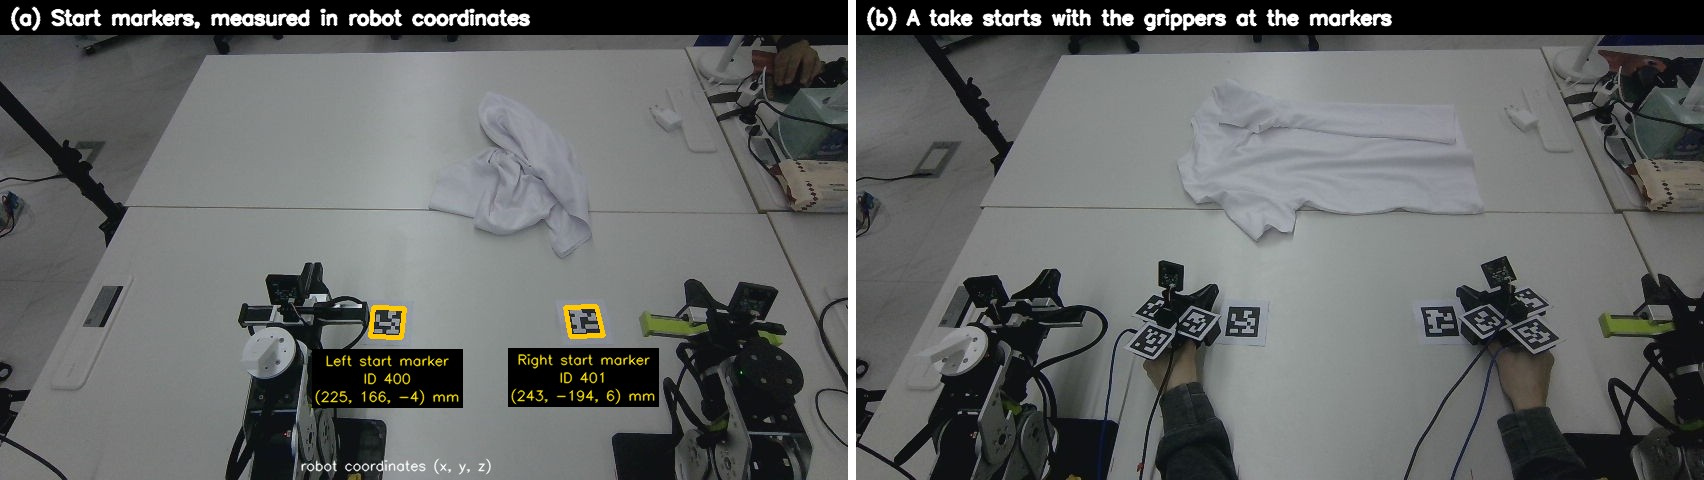
\includegraphics[width=0.92\textwidth]{figures/fig_start_markers.jpg}
\caption{Start markers. (a) Two AprilTags taped on the table (IDs 400 left, 401 right, 60\mm), measured once with the
calibrated Orbbec; their centres in robot coordinates are shown. (b) Every take starts with the two grippers at these
markers, so each demonstration begins at known robot coordinates.}
\label{fig:start}
\end{figure*}
Human and robot data use one world frame: the robot base frame $B$ of the right arm. It is set up in four steps, all once
per installation:
\begin{enumerate}
\item \emph{Camera to robot.} The robot moves the wrist calibration marker through 32 poses in front of the fixed Orbbec,
  which gives $T_{CB}$ (Sec.~\ref{sec:camrobot}). From then on every pose the camera measures can be written in $B$:
  $T_{B\cdot}=T_{BC}\,T_{C\cdot}$ with $T_{BC}=T_{CB}^{-1}$. The left arm base is located in the same frame by a second
  solve (Sec.~\ref{sec:corr}).
\item \emph{Start markers.} The two start markers on the table are measured once with the calibrated camera (PnP + depth,
  51 frames; Fig.~\ref{fig:start}a, Table~\ref{tab:cal}).
\item \emph{Gripper markers.} The markers of each gripper (three, four since 10-23) are calibrated to its jaw tip (Sec.~\ref{sec:rig}), so the
  camera gives the jaw-tip position directly in $B$.
\item \emph{Start of every take.} Each take starts with the grippers at the start markers (Fig.~\ref{fig:start}b), so every
  demonstration begins at the same known robot coordinates.
\end{enumerate}
No per-take alignment (no SLAM map, no point-cloud registration) is needed: a camera measurement of a gripper marker is
already a robot-frame pose.

The one-time calibration is the side input of the data chain (Fig.~\ref{fig:pipe}): it defines the shared world frame,
the robot base frame, and enters the chain at D1$\to$D2, D2$\to$D3 and the IK. Table~\ref{tab:cal} collects the results; their accuracy is discussed in
Sec.~\ref{sec:rescal}.

\begin{table}[t]
\caption{Calibration results}\label{tab:cal}
\centering\small
\begin{tabular}{@{}p{0.36\columnwidth}p{0.56\columnwidth}@{}}
\toprule
item & result \\
\midrule
Orbbec $\leftrightarrow$ robot base & 18/32 poses, held-out 0.98\,px, 1.3\mm lateral; human vs robot axes 1--6$^\circ$ \\
Robot TCP & URDF tip 89\mm off $\to$ $-0.019$\,m from gripper link; READY tip within 6--9\mm of tape \\
Left arm base & 70\mm inward, $\approx$3$^\circ$ tilt (1.6\,px, held-out 1.9\,px) \\
Left j2 & $-8.4^\circ$ offset, 3 poses within 5--10\mm \\
Start markers 400/401 & centres $(225, 166, -4)$\mm and $(243, -194, 6)$\mm \\
UMI tag rig $\to$ jaw tip & static 1--4\mm, leave-one-out 1.8--4.8\mm \\
UMI $\to$ robot gripper orientation & spread R 2.3$^\circ$, L 3.8--8.6$^\circ$ \\
IMU $\leftrightarrow$ Orbbec (rig) & time offset R 15 / L 10\,ms \\
Wrist cam $\leftrightarrow$ IMU & offset R $-40$ / L $-35$\,ms; rotation from data \\
Wrist cam $\to$ TCP & translation by tape, rotation solved \\
\bottomrule
\end{tabular}
\end{table}

\subsection{Notation}
$T_{XY}\in SE(3)$ maps coordinates in frame $Y$ to frame $X$; $R_{XY}$ and $t_{XY}$ are its rotation and translation.
Frames: $B$ robot base, $C$ Orbbec colour camera, $G$ gyro integration frame, $I$ IMU, $E$ robot TCP, and per UMI a rig
frame (tag 200 or 210) with tags $i$. The robot base frame follows the reBot URDF of the right arm: $+X$ forward, $+Y$
left, $+Z$ up, table at $z_\mathrm{t}=3$\mm. The jaw-tip TCP is the midpoint between the jaw tips on both sides, for the
UMI and for the robot. The jaw signal is $g=1$ open, $g=0$ closed.

\subsection{Camera to robot base}\label{sec:camrobot}
With the wrist calibration marker (ID 220) on the robot, the robot holds 32 poses $q_k$ around READY while the Orbbec records. For each hold, the tag
corners are taken as the median over the frames of the hold. The unknowns $T_{CB}$ and $T_{E,220}$ satisfy
\begin{equation}
T_{C,220}(k)=T_{CB}\,T_{BE}(q_k)\,T_{E,220},
\end{equation}
where $T_{BE}(q_k)$ is the forward kinematics. They are initialised with the method of Shah~\cite{shah2013robotworld} and
refined by minimising the reprojection error of all tag corners (Huber, 2\,px) plus a residual between the predicted tag
depth and the aligned Orbbec depth; at about 1\,m range the PnP depth of a 48--50\mm tag alone was too noisy to start from. The
solution is checked by five-fold held-out validation. The right-arm $T_{CB}$ defines the world frame.
\par\noindent\fbox{\parbox{0.96\linewidth}{\small\textbf{v0.1 status: the camera was raised twice (96$\to$105$\to$113\,cm) for the flattening takes. After each move $T_{CB}$ is
re-solved without moving the robot: the two fixed 70\mm table tags 400/401 (known robot coordinates) fix position and yaw,
and the table plane in the depth image fixes tilt and height (\code{scripts/robot_cam_from_anchors.py},
\code{robot_cam_v002}--\code{v005}). The 32-pose solve above produced \code{v001}.}}}\par

\subsection{Robot model corrections measured in the world}\label{sec:corr}
Three errors of the robot model were found only by measuring the real robot:
\begin{itemize}
\item \emph{TCP:} the URDF gripper TCP (gripper link + 70\mm) lies 89\mm in front of the real jaw tips, found with a tape
  measure at READY (tip 360\mm forward of the base centre, 280\mm above the table). The TCP is set to $-19$\mm from the
  gripper link. Every earlier absolute replay put the real jaws short by this offset along the tool axis; FK-versus-FK parity could not see it.
\item \emph{Left arm base:} solving $T_{CB}$ a second time with the tag on the \emph{left} wrist showed the left base 70\mm
  inward of the URDF with a 3$^\circ$ tilt. It is applied as a correction $D$ of the left \texttt{joint1} placement.
\item \emph{Left j2:} model joint = bridge joint + offset; a j2-only fit on READY and two further tape-measured poses gives
  $-8.4^\circ$.
\end{itemize}
All three are applied as overrides inside the IK model; the URDF file is untouched.

\subsection{UMI tag rig}\label{sec:rig}
Slow rotation takes give the tag-to-tag transforms $T_{\mathrm{rig},i}$ of each rig: each detection is solved with IPPE,
and $T_{\mathrm{rig},i}$ is a robust mean over good co-visible frames (chordal mean of the rotations, median of the
translations), chained through a common tag when two tags are never seen together. The jaw-tip position $t_\mathrm{tcp}$ in
the rig frame comes from touching the corners of a board of known geometry (16 holds per hand):
\begin{equation}
t_\mathrm{tcp}=\argmin_{t}\sum_{j}\rho\big(\lVert p_{B,\mathrm{rig}}(j)+R_{B,\mathrm{rig}}(j)\,t-c_B(j)\rVert\big),
\end{equation}
with $\rho$ a Huber loss (scale 5\mm) and $c_B(j)$ the touched corner. A pivot take (jaw tip held on one point while the
hand is tilted by about 50$^\circ$) gives a second, independent estimate.

\subsection{Other calibrations}\label{sec:othercal}
The UMI-to-robot-gripper orientation $R_{UE}$, used by the planner, comes from a take in which the UMI is held parallel to
the robot gripper at READY. The remaining two are used only by the optional SLAM filler (Sec.~\ref{sec:gaps}). The time
offsets between wrist camera and IMU and the camera--IMU rotation are estimated from data (MASt3R rotation rates against
the gyro); the Kalibr rotation from September was 173$^\circ$ off for the current right mount. The wrist-camera-to-TCP
translation is taped (right $(-5, 34, 122)$\mm, left $(-15, 14, 118)$\mm) and only the rotation is solved; a joint solve
that gave a 159\mm optical-axis offset was rejected.

% =====================================================================
\section{From UMI Data to Robot Motion}\label{sec:conv}
This section follows the data chain of Fig.~\ref{fig:pipe} for one take, one subsection per transformation.

\subsection{Recording: demonstration $\to$ D0}\label{sec:rec}
\emph{Input:} a human demonstration with both UMIs. \emph{Output:} D0, the raw recording on one clock.

One recorder writes the Orbbec colour and aligned depth (15\,Hz), both wrist videos (30\,Hz) and both IMUs. A spoken
protocol structures each take: the start pose with both UMIs at the start markers (Fig.~\ref{fig:start}b), then the
demos (each: hold, 30\,s of free motion, hold), then a final hold. Starting at the start markers puts every take in the
shared world frame (Sec.~\ref{sec:world}); the protocol cues define the demo windows used by all later transformations.
Every stream is stamped with the host monotonic clock; IMU device time is mapped to host time by a fitted clock model.
The replay later logs the commanded and the measured joints on the same clock, so no synchronisation hardware is needed.

\subsection{Tag detection: D0 $\to$ D1}\label{sec:tagdet}
\emph{Input:} the Orbbec colour and depth frames of D0. \emph{Output:} D1, the pose of every visible tag per frame in the
camera frame.

Tags with a pixel side under 18\,px are ignored. Each remaining tag $i$ is solved with IPPE, giving $T_{C,i}$ and its
centre $c_i$. If the median Orbbec depth $d_i$ inside the tag quadrilateral is valid and within 0.10\,m of $c_{i,z}$, the
centre is moved along its ray: $c_i\leftarrow c_i\,d_i/c_{i,z}$. At about 1\,m range, depth is the least accurate PnP coordinate.

\subsection{UMI tag rig: D1 $\to$ D2}\label{sec:rigpose}
\emph{Input:} D1 and the calibrated tag rig $T_{\mathrm{rig},i}$ (Sec.~\ref{sec:rig}). \emph{Output:} D2, the rig pose
$T_{C,\mathrm{rig}}$ of each UMI per frame in the camera frame.
\begin{enumerate}
\item \emph{Rig pose from the tags.} With one visible tag, $T_{C,\mathrm{rig}}=T_{C,i}T_{\mathrm{rig},i}^{-1}$. With two or
  more, all corners $X_{ik}=T_{\mathrm{rig},i}\,x_k$ are solved jointly,
  \begin{equation}
  T_{C,\mathrm{rig}}=\argmin_{T}\sum_{i,k}\lVert \pi(K,T X_{ik})-u_{ik}\rVert^2,
  \end{equation}
  initialised with SQPnP and refined with Levenberg--Marquardt. Frames with reprojection RMSE above 2\,px are dropped.
\item \emph{Rotation.} Either from the tags, or from the gyro anchored to the tags:
  \begin{equation}
  R_{C,\mathrm{rig}}(t)=\bar R_{CG}(t)\,R_{GI}(t)\,R_{I,\mathrm{rig}},
  \end{equation}
  where $R_{GI}$ integrates the gyro minus its bias (median over still samples), $R_{I,\mathrm{rig}}$ is calibrated, and
  $\bar R_{CG}(t)$ is the weighted rotation mean of $R^\mathrm{tag}_{C,\mathrm{rig}}R_{I,\mathrm{rig}}^\top R_{GI}^\top$
  over tag frames within $\pm10$\,s (weight 1 with two or more tags, 0.15 with one).
\item \emph{Position.} $p_{C,\mathrm{rig}}=\frac{1}{|V|}\sum_{i\in V}\big(c_i-R_{C,\mathrm{rig}}\,t_{\mathrm{rig},i}\big)$
  over the visible tags $V$; using the fused rotation removes the leak of single-tag rotation error into position.
\end{enumerate}

\subsection{Jaw tip in the robot base frame: D2 $\to$ D3}\label{sec:tcp}
\emph{Input:} D2, the jaw-tip offset $t_\mathrm{tcp}$ (Sec.~\ref{sec:rig}) and $T_{BC}$ (Sec.~\ref{sec:camrobot}).
\emph{Output:} D3, the human jaw-tip TCP trajectory in the robot base frame, with gaps where no tag is seen.
\begin{align}
p_B&=R_{BC}\big(R_{C,\mathrm{rig}}\,t_\mathrm{tcp}+p_{C,\mathrm{rig}}\big)+t_{BC},\\
R_{B,\mathrm{tcp}}&=R_{BC}R_{C,\mathrm{rig}}.
\end{align}
No per-take alignment is applied: the start markers place the start of every take in the robot base frame.

\subsection{Gap filling and jaw state: D3 (+ D0) $\to$ D4}\label{sec:gaps}
\begin{figure*}[!t]
\centering
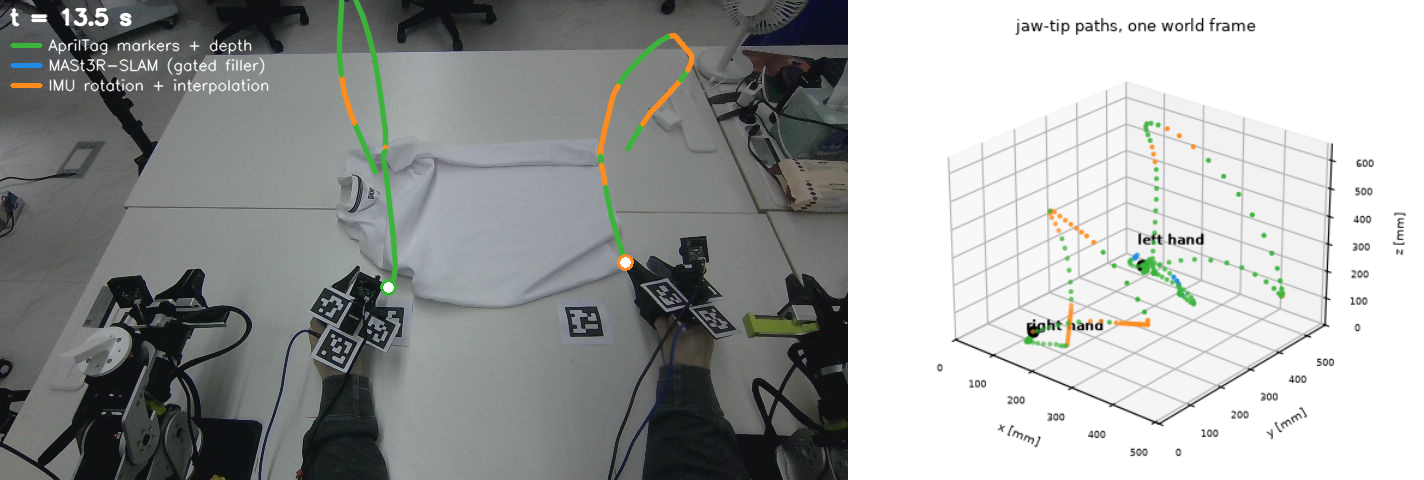
\includegraphics[width=0.92\textwidth]{figures/fig_trajectory_sources.png}
\caption{Reconstructed jaw-tip trajectories D4 of demo~2 (take 171057), one frame of the animation in \texttt{media/}.
Left: the last 3\,s of both paths projected into the Orbbec image, coloured by the source of each frame: AprilTag markers
+ depth (green), MASt3R-SLAM filler (blue), IMU rotation + interpolation while the markers are hidden (orange). Right:
both paths up to this time in the robot base frame (offset to the workspace corner). Orange appears exactly when a hand
grasps or lifts the cloth.}
\label{fig:trajsrc}
\end{figure*}
\par\noindent\fbox{\parbox{0.96\linewidth}{\small\textbf{v0.1 status: superseded for training data on 10-24. Position now comes from fixed-camera point tracking fused with the
tags (Sec.~\ref{sec:trainpose}); MASt3R-SLAM is not used, and its code moved to \code{legacy/scripts/mast3r_gapfill/} and
\code{legacy/slam/mast3r/}. The binary jaw classifier below is now followed by a jaw-tip keypoint model that gives a
continuous aperture. This subsection is kept for the replay track.}}}\par
Figure~\ref{fig:trajsrc} shows which source supplies each frame of a full demonstration.
\emph{Input:} D3, the IMU and the wrist video of D0. \emph{Output:} D4, a continuous human trajectory with jaw-tip pose and
jaw state per frame in the robot base frame.

\textbf{IMU.} Frames without a tag get the gyro-anchored rotation of Sec.~\ref{sec:rigpose} and a linearly interpolated
position, and are flagged ($n_\mathrm{tags}=0$) as not measured.

\textbf{Optional MASt3R-SLAM filler.} MASt3R-SLAM~\cite{murai2025mast3rslam} runs on the wrist video undistorted to a
960$\times$540 pinhole image. The official loop does not recover after a tracking loss, so our runner restarts it on
consecutive segments; each segment is its own world. For each segment a Sim(3) to the tag path is fitted on
\emph{alignment} tag frames, and \emph{validation} tag frames (1\,s of every 4\,s) never enter the fit. A segment is kept
only if its scale is in $[0.05, 3]$, after a tail cut on growing residuals, and if it stays within 0.15\,m of the tag/IMU
path. The fused path uses SLAM where kept and the tag/IMU path elsewhere, smoothed by a 5-frame moving average. Four
numbers decide its value: coverage, survival at grasps (tag-hidden frames within $\pm$1.5\,s of a jaw event that have a
SLAM pose), error on validation frames, and the jump where two kept segments meet (Sec.~\ref{sec:slam}). The camera--IMU
and camera-to-TCP calibrations it needs are in Sec.~\ref{sec:othercal}.

\textbf{Jaw state.} An ImageNet-pretrained ResNet-18 per hand classifies a fixed region of the wrist fisheye that shows the
bare jaws (bottom centre; the left ROI is lower because that camera sees the jaws only in the bottom 30\% of the image).
The crop is resized to 224$\times$224. Training uses spoken open/closed capture cycles with brightness, contrast, gamma,
shift and blur augmentation, AdamW, and validation on held-out cycles. The output $p_\mathrm{open}$ is thresholded with
hysteresis: right 0.3/0.1, left 0.6/0.4. The left images are washed out, and closed frames score 0.2--0.35; with the
right-hand thresholds the left jaw appeared ``reversed''.

\subsection{Robotization: D4 $\to$ D5}\label{sec:robotize}
\emph{Input:} D4. \emph{Output:} D5, a robot-feasible jaw-tip trajectory, with the human path kept next to it and a
per-frame quality label.
\par\noindent\fbox{\parbox{0.96\linewidth}{\small\textbf{v0.1 status: kept for the replay track. The training label A (Sec.~\ref{sec:trainlabels}) keeps the fused path in reBot
gripper axes with 0.25\,s smoothing and the table clearance, and does not take the IK result back. The per-frame quality
labels 0/1/2 below are replaced by per-demo grades (Sec.~\ref{sec:trainquality}).}}}\par

The human path is changed only by continuous warps, never by clipping. Per demo window and hand, let $y$ be the lateral
coordinate and $d$ the minimum hand separation (\texttt{-{}-sep}, 0.06\,m). For the right hand, with $y_o$ and $y_i$ the
1st and 99th percentiles of $y$,
\begin{align}
s&=\begin{cases}1, & y_i\le -d/2,\\ \clip\!\big(\tfrac{-d/2-y_o}{y_i-y_o},\,0.4,\,1\big), & \text{otherwise,}\end{cases}\\
y'&=\mathrm{softceil}\big(y_o+s\,(y-y_o),\;-d/2,\;w\big),
\end{align}
and the left hand is mirrored. The height gets a soft floor,
\begin{align}
z'&=\mathrm{softfloor}(z,\,z_\mathrm{t}+c,\,w),\\
\mathrm{softfloor}(z,f,w)&=f+w\log\!\big(1+e^{(z-f)/w}\big),
\end{align}
with $\mathrm{softceil}(y,c,w)=-\mathrm{softfloor}(-y,-c,w)$, $w=10$\mm and clearance $c=0$. The softplus floor also lifts
points that lie exactly at the floor by $w\ln2\approx7$\mm. The $y$ compression addresses hands that cross the body
midline and come within 3--11\,cm of each other (seen in take 113243); the floor addresses tag TCPs below the table. An
optional minimum reach from each arm base is off.

The displacement $\delta=\lVert p'_B-p_B\rVert$ of each frame is stored with a quality label: 0 for $\delta<20$\mm, 1 for
$<$50\mm, 2 otherwise. Training will use the robot-feasible path with these labels as weights; large shifts in contact
phases are the harmful ones.

\subsection{Limit-aware IK: D5 $\to$ D6}\label{sec:plan}
\emph{Input:} D5, the jaw state of D4 and the robot model with the overrides of Sec.~\ref{sec:corr}. \emph{Output:} D6, a
joint trajectory for the $2\times6$ joints plus jaw commands at 30\,Hz.
\par\noindent\fbox{\parbox{0.96\linewidth}{\small\textbf{v0.1 status: the same IK (wrist-roll relaxation, jaw flip, step bound) now runs offline only as a checker of the
training labels (Sec.~\ref{sec:trainlabels}); the policy is executed by the online loop of Sec.~\ref{sec:deploy}.}}}\par

\textbf{Target.} For each command sample the target is
\begin{equation}
T^\star=\Big(\,R_{B,\mathrm{tcp}}(t)\,R_{UE}\,R_z(\pi)^{f}\,R_z(\varphi)\;,\;p'_B(t)\Big),
\end{equation}
where $R_{UE}$ is the UMI-to-robot-gripper orientation (Sec.~\ref{sec:othercal}), $f\in\{0,1\}$ the jaw flip and $\varphi$
the relaxed wrist roll (below). The human time is resampled to the command rate (30\,Hz) at the replay speed, and
positions are smoothed by a 15-sample moving average on that grid.

\textbf{IK.} Pink~\cite{pink} solves a differential IK QP per iteration with a frame task on the TCP (position cost 1,
orientation cost 0.1, so position comes first), a weak posture task toward the seed (cost $10^{-3}$), and the joint limits
of the bridge, shifted by the joint offsets and tightened by 0.5$^\circ$.
\begin{itemize}
\item \emph{Step bound.} The first frame is solved freely from READY; for every later frame the accumulated change of each
  joint is box-projected to $\lvert q_j-q_j^{\mathrm{prev}}\rvert\le5^\circ$. Without this bound, j6 reaching its
  $\pm130^\circ$ limit made the IK jump to another solution (2500$^\circ$/s).
\item \emph{Wrist-roll relaxation.} j6 turns about the tool axis, on which the TCP lies, so a roll $\varphi$ about that axis
  moves j6 by about $\varphi$ without moving the TCP. With threshold $\theta=115^\circ$ and $q_6$ the solved j6,
  \begin{equation}
  \varphi\leftarrow\begin{cases}\varphi-\sgn(q_6)\,(\lvert q_6\rvert-\theta), & \lvert q_6\rvert>\theta,\\
  \varphi-\sgn(\varphi)\min\big(\lvert\varphi\rvert,1^\circ,\theta-\lvert q_6\rvert\big), & \text{otherwise.}\end{cases}
  \end{equation}
  Position is never traded.
\item \emph{Jaw symmetry.} The parallel jaw is symmetric under 180$^\circ$ about the tool axis. Both $f=0$ and $f=1$ are
  planned, and the one with fewer frames above 10\mm IK error (then the smaller maximum error) is used.
\item \emph{Finger-corner clearance.} With $x_E,y_E$ the tool axes, the lowest corner of the fingers is estimated as
  \begin{equation}
  z_\mathrm{low}=z_\mathrm{tcp}-h\,\lvert x_{E,z}\rvert-(a+b\,g)\,\lvert y_{E,z}\rvert,
  \end{equation}
  with $h=20$\mm (half finger length along the tool $x$), $a=8$\mm, $b=28$\mm and $g$ the jaw opening from the classifier.
  If $z_\mathrm{low}<z_\mathrm{t}+c_\mathrm{tip}$, the target is raised by the difference. The default is
  $c_\mathrm{tip}=+5$\mm (from the first cloth grasp, Sec.~\ref{sec:resgrasp}); the full two-arm replays use
  $c_\mathrm{tip}=-10$\mm (Sec.~\ref{sec:jawheight}).
\item \emph{Floor.} Targets below $z_\mathrm{t}+10$\mm are raised to it and counted.
\end{itemize}
The joint path is smoothed by a 9-sample moving average. Approach and retreat legs connect READY to the path in Cartesian
space (READY $\to$ above the start $\to$ start, end $\to$ above the end $\to$ READY; the short descent onto the start is a
joint-space line); a joint-space line between far poses had taken links under the table.

\textbf{Jaw commands.} At 600$^\circ$/s jaw speed the robot jaw reaches half travel 331--337\,ms after its command (no load;
at the earlier 90$^\circ$/s it took 1969\,ms). Jaw commands are therefore placed before the human event: open by 320\,ms
and close by 480\,ms. These leads were set from a gripper-only replay so that the robot jaw is at 50\% when the human jaw
is at mid-stroke (the classifier's open event fires near mid-stroke, its close event about 150\,ms after it), and verified
on a second run (robot 50\% at the open event $+4$\,ms, at the close event $-171$\,ms for a target of $-150$\,ms). At replay
speed $s$, a lead $L$ in robot time is a lead $sL$ in human time.

\subsection{Safety checks: D6 $\to$ approved plan}\label{sec:checks}
\emph{Input:} D6. \emph{Output:} the same plan, approved for execution, or a rejection.

The plan must pass all of these before \texttt{-{}-go}: maximum IK position error and rotation deviation, joint limits,
joint speed, TCP height, height of links 3--6, gripper and fingers above the table, and a minimum distance of 120\mm
between any link origin of the left arm and any of the right arm (every 5th step and along the approach and retreat legs).
A regression test re-plans the right-arm grasp window of the first cloth grasp and fails if IK error, joint speed, link
clearance or arm gap get worse.

\subsection{Execution: approved plan $\to$ D7}\label{sec:replay}
\emph{Input:} the approved plan. \emph{Output:} D7, the robot motion (commanded and encoder joints) on the host clock.

Commands stream at 30\,Hz to the 100\,Hz MIT-mode bridge (Sec.~\ref{sec:bridge}); at speed 0.35 a 33\,s demo takes 94\,s.
The log stores, for each command, its human source time, so every robot sample can be mapped back to the demonstration.

% =====================================================================
\section{Experimental Setup}\label{sec:setup}
\subsection{Data and runs}\label{sec:data}
\begin{itemize}
\item \emph{Single-arm parity} (10-20): stroke takes with six translation directions, rotation strokes and free combined
  motion, replayed on one arm.
\item \emph{Take 113243}, demo~1: the first cloth grasp (right arm, grasp window 19.5--24\,s), the robotization example of
  crossing hands, and the SLAM tests.
\item \emph{Take 171057}, demo~2 (33\,s): the full two-arm replay (10-21) and the SLAM tests. Conversion without hand
  edits: tag + depth pose, MASt3R fill where it agrees, robotization with $d=0.06$\,m and $c=0$. Runs: 190154 (stopped
  early), 193127 (planner default $c_\mathrm{tip}=+5$\mm), then 194526, 195154, 195745 and 200335 with one unchanged plan
  ($c_\mathrm{tip}=-10$\mm).
\end{itemize}

\subsection{Metrics and parity gates: D7 vs.\ D4/D5}\label{sec:eval}
The replay is compared at three levels: A is the human jaw-tip TCP from tags (D4), B the robot command (FK of
the commanded joints of D6), C the robot (FK of the encoder readings of D7). When the replayed path was robotized (the
two-arm replay), the reference is the robotized path A$'$ (D5) that was replayed instead of A. For a free-motion window:
\begin{itemize}
\item A is taken relative to the median pose of the hold before the motion, B and C relative to their first sample;
\item C is shifted in time by the lag $L^\star$ that minimises the mean of $\lVert C(t+L)-B(t)\rVert^2$ (searched over
  0--1.5\,s in 20\,ms steps), so that lag is not counted as error;
\item position error $e_p(t)=\lVert C(t+L^\star)-A(t)\rVert$, reported as RMSE and p95; rotation error is the geodesic
  angle between the relative rotations of C and A, reported as median and p95;
\item amplitude ratios (RMS distance from the start, C over A), C$-$B and B$-$A RMSE, and a count of jumps.
\end{itemize}
\textbf{Gates.} RMSE $<$20\mm, p95 $<$30\mm, rotation median $<$5$^\circ$ and p95 $<$10$^\circ$, ratios 0.9--1.1, no jumps.
Single-axis strokes are compared on normalised progress along A's chord instead, with gates on the main-axis ratio
(0.9--1.1), cross-axis leakage ($<$10\%), endpoint ($<$20\mm), RMSE and p95. Jaw timing is compared on the normalised phase
of the window (UMI event, command, encoder crossing). For the full two-arm replay the whole demo is one window.

\subsection{Video alignment}\label{sec:video}
The same Orbbec films the replay, and the stored mapping from command time to human time produces frame-aligned
side-by-side videos (Fig.~\ref{fig:sbs}), in human time or, with \texttt{-{}-robot-time}, in robot time.

% =====================================================================
\section{Results}\label{sec:res}
\subsection{Calibration accuracy}\label{sec:rescal}
Table~\ref{tab:cal} gives the calibration results. The camera-to-robot solve reaches 0.98\,px and 1.3\mm lateral error on
held-out poses (18 of 32 poses used). The tag rig places the jaw tip with 1--4\mm static error; leaving one board corner
out gives 1.8--4.8\mm, and the independent pivot take leaves a residual RMS of 6.7\mm (right) and 5.3\mm (left). The
absolute jaw position of the corrected robot model agrees with tape measurements within 6--9\mm at READY, and the left
j2 fit within 5--10\mm at its three poses (residuals $\le$8\mm, RMS 4.8\mm). The UMI-to-robot-gripper orientation has a
spread of 2.3$^\circ$ (right) and 3.8--8.6$^\circ$ (left).

\subsection{Single-arm parity (10-20)}\label{sec:res1arm}
\begin{itemize}
\item Six-direction translation strokes: 16/18 pass; median RMSE $X$ 11.6, $Y$ 7.3, $Z$ 5.5\mm (max 14.5\mm); robot
  endpoint repeatability $\le$8\mm. The two failures were a marginal cross-axis leak (11.1\%) and one bad human stroke.
\item Gain history: earlier settings, starting from $K_p$ 64 and $K_i$ 28, had passed 0/6, 3/6 and 5/6 strokes. Raising
  $K_i$ from 28 to 56 on all joints, then to 84 on j2, reduced the $X$-stroke RMSE from 25/37\mm to 17/16\mm and then to
  14/12\mm (Sec.~\ref{sec:bridge}).
\item Rotation strokes: ratio 0.98--1.04, geodesic median 0.3--1.6$^\circ$, repeat $\le$1.4$^\circ$.
\item Free combined motion at 0.9$\times$: 2/2 pass (RMSE 13.7/14.6\mm, p95 26/29\mm, rotation median 1.7/1.4$^\circ$,
  ratios 0.99--1.03, robot lag about 0.2\,s).
\item In these tests B$-$A was at most 3.4\mm; the error was robot tracking (C$-$B).
\item The jaw command follows the human jaw event within 0.5\% of progress.
\end{itemize}

\subsection{First cloth grasp (10-21)}\label{sec:resgrasp}
After the TCP fix (Sec.~\ref{sec:corr}), the right arm replayed the grasp window of demo~1 of take 113243 and picked up and
lifted the T-shirt. The first attempt scraped the table at a 46$^\circ$ tool tilt, which led to the finger-corner clearance
with $c_\mathrm{tip}=+5$\mm (Sec.~\ref{sec:plan}).

\subsection{Two-arm replay of a full demo (10-21)}\label{sec:resbi}
\textbf{Input.} In the demo window of take 171057, demo~2, the right hand had at least one tag in 79\% of the frames and
the left hand in 95\%; 21\% of the right-hand frames had neither a tag nor a kept SLAM pose and are interpolated.
Robotization did not compress $y$ in this demo (each hand stayed on its side); only the table floor acted. The per-frame
displacement had a median of 0.1\mm (right) and 1.1\mm (left), a p95 of 9.3 and 20.6\mm, and a maximum of 10.5 and
21.5\mm; all right-hand frames and 92\% of the left-hand frames are in quality class 0, the rest in class 1
(Fig.~\ref{fig:robotize}).

\begin{figure*}[!t]
\centering
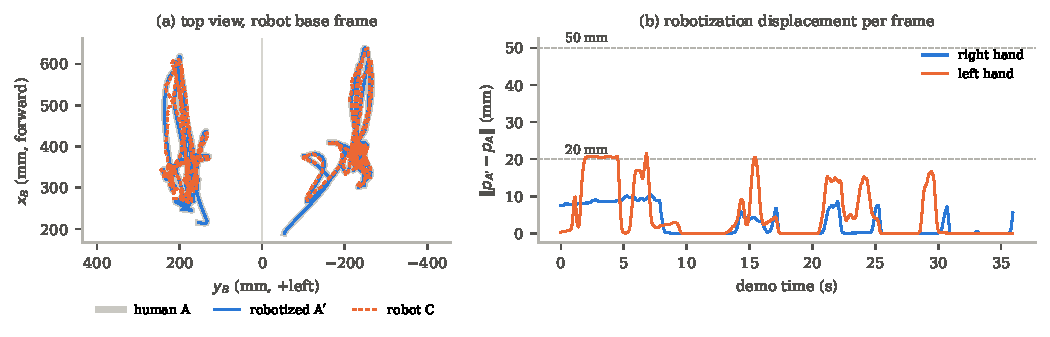
\includegraphics[width=0.9\textwidth]{figures/fig_robotize.pdf}
\caption{Demo~2 of take 171057 and run 200335. (a) Top view of the human TCP (A, wide gray), the robotized target (A$'$)
and the robot from encoders (C) for both hands in the robot base frame; A and A$'$ coincide in $xy$ because only the height
was warped. (b) Robotization displacement per frame; the dashed lines are the 20 and 50\mm quality thresholds. Computed
from \texttt{umi\_traj\_*\_fused\_robot.npz} and the replay log.}
\label{fig:robotize}
\end{figure*}

\textbf{Plan.} IK error at most 6.3\mm/11.5$^\circ$ (right) and 10.3\mm/21.0$^\circ$ (left), joint speed $\le$88$^\circ$/s,
lowest TCP target 13\mm (commanded TCP 4\mm after the joint smoothing), lowest link 1--5\mm above the table, arm-to-arm link distance $\ge$269\mm.

\begin{table*}[t]
\caption{Two-arm replay of demo 2 against the replayed, robotized human path A$'$ (D5), per run (whole demo as one window)}\label{tab:rep}
\centering\small
\begin{tabular}{@{}llcccccccc@{}}
\toprule
run & arm & human range & pos.\ RMSE & pos.\ p95 & rot.\ median & rot.\ p95 & endpoint & C$-$B & B$-$A$'$ \\
\midrule
194526 & right & 464\mm / 40$^\circ$ & 17.2\mm & 36.8\mm & 8.1$^\circ$ & 12.6$^\circ$ & 20\mm / 9.7$^\circ$ & 12.1\mm & 8.6\mm \\
194526 & left & 572\mm / 56$^\circ$ & 29.8\mm & 51.0\mm & 12.6$^\circ$ & 17.1$^\circ$ & 19\mm / 16.2$^\circ$ & 14.5\mm & 22.6\mm \\
195154 & right & & 17.3\mm & 36.8\mm & 8.1$^\circ$ & 12.7$^\circ$ & 20\mm / 9.8$^\circ$ & 12.2\mm & 8.6\mm \\
195154 & left & & 30.3\mm & 49.5\mm & 12.7$^\circ$ & 17.0$^\circ$ & 19\mm / 16.0$^\circ$ & 15.2\mm & 22.6\mm \\
195745 & right & & 17.2\mm & 35.3\mm & 8.1$^\circ$ & 12.7$^\circ$ & 20\mm / 9.7$^\circ$ & 12.1\mm & 8.6\mm \\
195745 & left & & 29.0\mm & 49.8\mm & 12.3$^\circ$ & 17.2$^\circ$ & 18\mm / 16.0$^\circ$ & 15.2\mm & 22.6\mm \\
200335 & right & & 17.4\mm & 35.8\mm & 8.1$^\circ$ & 12.6$^\circ$ & 20\mm / 9.7$^\circ$ & 12.3\mm & 8.6\mm \\
200335 & left & & 30.3\mm & 51.3\mm & 12.7$^\circ$ & 17.2$^\circ$ & 21\mm / 16.0$^\circ$ & 15.5\mm & 22.6\mm \\
\bottomrule
\end{tabular}
\end{table*}

\textbf{Error against the human} (Table~\ref{tab:rep}): 17\mm RMSE right and 30\mm left against the replayed,
robotized path A$'$. Against the raw human path (D4) the same runs give 22\mm (right) and 32--34\mm (left), because the
robotization displacement (Fig.~\ref{fig:robotize}) then also counts as error. The four runs agree within about 1\mm, so
the robot is deterministic and the remaining error is systematic.
\begin{itemize}
\item \emph{Where the left error comes from:} the left command already deviates from A$'$ (B$-$A$'$ 22.6\mm, right
  8.6\mm); the left IK gives up to 21$^\circ$ of orientation. Against the raw human path, the larger left robotization
  adds to this.
\item \emph{Tracking:} the robot follows its own command with 12--16\mm RMSE over the path (C$-$B), and closely at the
  grasp moments (Sec.~\ref{sec:jawheight}, Fig.~\ref{fig:z}).
\end{itemize}

\begin{figure}[!t]
\centering
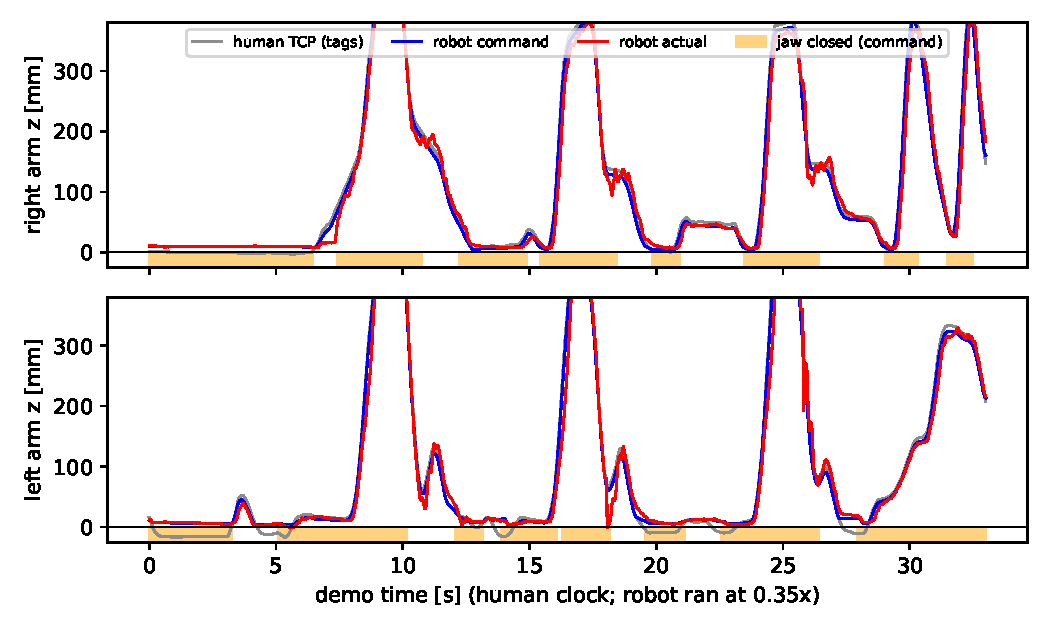
\includegraphics[width=\columnwidth]{figures/fig_z_trace.pdf}
\caption{Height of the human TCP (tags), the robot command and the robot (encoders) over the demo (run 200335). Orange:
jaw closed. The robot follows the robotized path closely; near the table the command sits slightly above the human because
of the soft table floor.}
\label{fig:z}
\end{figure}

\subsection{Jaw height at the grasp}\label{sec:jawheight}
In the first full replays (run 193127, $c_\mathrm{tip}=+5$\mm) the jaws closed 19--61\mm above the table and missed the
cloth. The cause was the finger-corner clearance: with the tool tilted, the open fingers' lowest corner is 20--36\mm below
the TCP, so the planner lifted the TCP.
\begin{itemize}
\item \emph{Allowing the corner to touch} ($c_\mathrm{tip}=-10$\mm), as the human's fingers do, moves the near-table closes
  to 14--16\mm (right, 4 closes) and 5--19\mm (left, 5 closes), with an $xy$ error of 2--8\mm against the command at that
  moment (run 194526, Fig.~\ref{fig:close}). Every link stays at least 1\mm above the table.
\item \emph{Tilting the tool toward vertical instead} (only where the corner would touch) was tried: the IK could not
  follow even 15$^\circ$ (errors up to 100\mm).
\item \emph{Closing at the lowest point} nearby, a heuristic, was rejected.
\end{itemize}

\begin{figure}[!t]
\centering
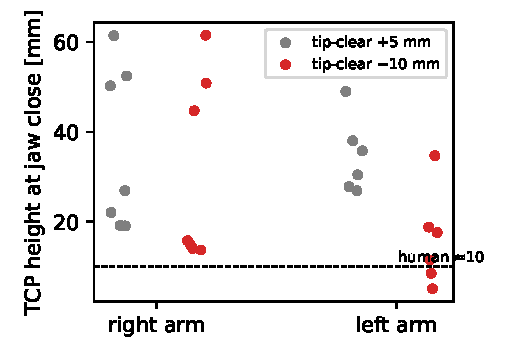
\includegraphics[width=0.62\columnwidth]{figures/fig_close_height.pdf}
\caption{TCP height at each jaw close, with the default finger-corner clearance ($+5$\mm, run 193127) and with the corner
allowed to touch ($-10$\mm, run 194526). The dashed line is the human ($\approx$10\mm).}
\label{fig:close}
\end{figure}

\textbf{Outcome.} In runs 195154 and 195745 the shirt lay 15--20\,cm farther away than in the demo, and the jaws closed on
the empty table. In run 200335 the jaws caught the shirt edge and dragged it (Fig.~\ref{fig:sbs}); the shirt was moved,
but not folded as by the human. The earlier full run 190154 stopped when the right arm lost power; its right-arm encoder
log ends 52\,s into the 94\,s replay.

\subsection{Negative results}\label{sec:neg}
\subsubsection{SLAM as the trajectory source}\label{sec:slam}
The tags are hidden exactly when the hand grasps, palm down, so wrist-camera SLAM was tested as the main path.
\begin{itemize}
\item \emph{MASt3R-SLAM} (restart runner of Sec.~\ref{sec:gaps}, Table~\ref{tab:slam}): where it tracks it is accurate
  (2--14\mm on validation frames), but it keeps only 19--48\% of the frames and 0--38\% of the tag-hidden frames around
  grasps. White cloth fills the view at close range and the hand moves fast; each restart starts a new world that needs tag
  anchors. On the earlier UMIalign takes it also drifted within segments: a single Sim(3) per segment left a median
  residual of 69\mm (9\mm with 2\,s windows), and the tilt drifted 5--12$^\circ$ over 10\,s.
\item \emph{ORB-SLAM3 mono-inertial}~\cite{campos2021orbslam3} (take 113243, both hands): initialised and gave accurate
  rotation, but the translation scale diverged 30--1000$\times$ (coverage 0--11\%, grasp survival 0\%). The hand's
  acceleration (median 0.07--0.16\,m/s$^2$) is below the accelerometer bias (0.25--0.43\,m/s$^2$), so the IMU cannot
  observe scale; white cloth at close range adds weak visual constraints.
\item \emph{Stereo VIO} (10-15/16, an earlier stereo camera): AirSLAM stereo-inertial diverged (15\,m range, 21\% lost
  frames); stereo VO alone ran with 3.6\% lost frames; Basalt and OpenVINS were also set up. The stereo camera was dropped
  on 10-16.
\end{itemize}
SLAM was therefore kept only as a gated filler in v0 (Sec.~\ref{sec:gaps}); in v0.1 it is not used at all.

\begin{table}[t]
\caption{MASt3R-SLAM on the wrist video (restart runner)}\label{tab:slam}
\centering\small
\begin{tabular}{@{}lcccc@{}}
\toprule
take / hand & kept & grasp survival & hidden err. & jump \\
\midrule
113243 right & 19\% & 0\% & 2.2\mm & 39.6\mm \\
113243 left & 28\% & 38\% & 13.9\mm & 72.9\mm \\
171057 right & 20\% & 12\% & -- & -- \\
171057 left & 48\% & 32\% & -- & -- \\
\bottomrule
\end{tabular}
\end{table}

\subsubsection{Earlier labels (10-13 to 10-16)}
Before the tag rig, a smoother fused MASt3R, Orbbec body tracking of the UMI and the IMU. It had three errors, all
invisible to its own quality checks (Orbbec residual, jumps, coverage):
\begin{itemize}
\item a stale Kalibr camera--IMU rotation (17--24$^\circ$ off);
\item a free camera-to-TCP lever that converged 20--35\,cm wrong (it had to be fixed from the jaw tips seen by the Orbbec);
\item dark sleeves taking over the body anchor (removed by a gate against the top AprilTag).
\end{itemize}
After fixing them, the TCP was still only 38--59\mm (median per session) from the jaw tape seen by the Orbbec. A 65-episode
``flatten and align'' set built from these labels was used to fine-tune a policy; it is not evaluated here. The 4--6\,cm
label error motivated the 1--4\mm tag rig.

% =====================================================================
\section{Training Data for Policy Learning (10-22 to 10-27)}\label{sec:train}
Open-loop replay (Secs.~\ref{sec:conv}--\ref{sec:res}) needs the cloth where the human's was. The next step is a policy
that sees the cloth. This section describes how 300 flattening demonstrations were turned into training data. The code is
in \code{processing/} of the repository (Appendix~\ref{app:repo}); Table~\ref{tab:stages} maps the stages.

\begin{table}[t]
\caption{Training-data stages (code in \texttt{processing/})}\label{tab:stages}
\centering\scriptsize
\begin{tabular}{@{}p{0.04\columnwidth}p{0.25\columnwidth}p{0.62\columnwidth}@{}}
\toprule
\# & stage & what \\
\midrule
1 & success & judged by eye on the frame 0.5\,s before each demo ends \\
2 & jaw state & classifier v003 (GPU) $\to$ YOLO-pose jaw tips $\to$ aperture $g$ \\
3 & tag pose & tags $\to$ TCP, per-take camera calibration (v002--v005) \\
4 & prep & arm assignment by table side, idle rows, start seeds, tag rotation \\
5 & point tracking & 40 query points per gripper, CoTracker3 online (GPU) \\
6 & 3-D + gates & depth lift, rigid fit, hidden-tag hold-out; gates G1--G3 \\
7 & fusion & variant Cg: points + tag anchors + bias; IMU only in gaps \\
8 & trims & idle trim (10\,cm/s, 0.3\,s) + edge-gap trim \\
9 & quality & GOLD / SILVER / REJECT; QA video per demo \\
10 & labels & A (before IK) for training, B (IK$\to$FK) for QA; IK diagnostics \\
11 & dataset & LeRobot v3, 20\,Hz, 3 cameras, state 30-D, action 20-D \\
12 & eval / deploy & offline k16/k32 eval; receding-horizon deploy \\
\bottomrule
\end{tabular}
\end{table}

\subsection{Collection}\label{sec:traincoll}
Each demo flattens a crumpled T-shirt on the table with both UMIs. 318 demos were recorded on 26 and 27 October and 300
were judged successful on the frame 0.5\,s before the demo ends (the operator re-crumples the shirt right after the end
key). Four shirts were used: beige 72, black 92, white 82 and blue 54 successful demos. The protocol is the same as in
Sec.~\ref{sec:rec}; the camera sits at 1.13\,m so that both hands stay in view. On the 10-22 and later takes the rig labels
were swapped against the wrist cameras, so each gripper track is assigned to an arm by its side of the table ($y$ in the
robot base), not by its label.

\subsection{Pose: point tracking, tags and IMU}\label{sec:trainpose}
\begin{figure*}[!t]
\centering
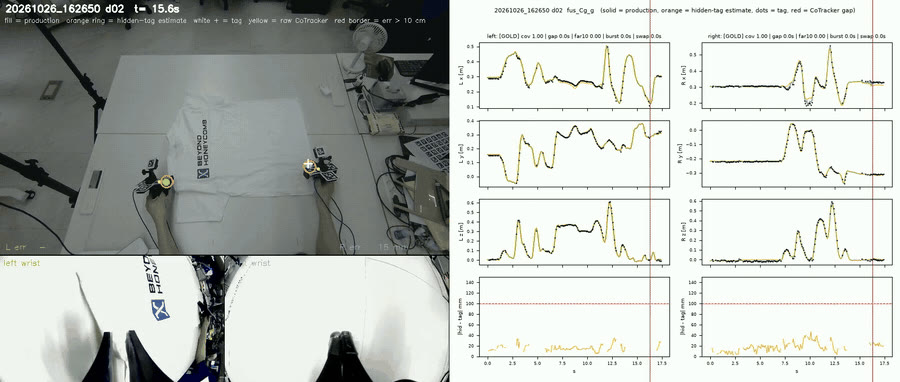
\includegraphics[width=0.92\textwidth]{figures/fig_fusion_qa.jpg}
\caption{Per-demo QA video of a GOLD demo (take 20261026\_162650, demo~2; one frame of \texttt{media/flatten\_fusion\_qa\_gold.gif}).
Top left: fixed camera with the fused jaw tips (filled dots), the estimate made with that tag hidden (orange ring), the tag
itself (white +) and raw CoTracker points (yellow). Bottom left: both wrist cameras. Right: $x$, $y$, $z$ of each hand over
time, and the hidden-tag error (bottom row; red dashed line = 10\,cm).}
\label{fig:fusqa}
\end{figure*}
Tags are hidden whenever the cloth or the other hand covers them, which is exactly at grasps. The position therefore comes
from point tracking on the fixed camera, with the tags as anchors:
\begin{enumerate}
\item \emph{Points.} CoTracker3~\cite{karaev2024cotracker3} (online mode) follows 40 query points per gripper through the
  Orbbec colour video, seeded on the gripper body at the start of each demo.
\item \emph{3-D.} The aligned depth lifts the points to 3-D, and a rigid gripper model fitted to them gives the gripper
  body centre per frame. The fit is repeated with the tags of every third block hidden (hold-out runs).
\item \emph{Gates.} A frame is marked invalid when G1 the track acceleration disagrees with the IMU acceleration
  (normalised cross-correlation $<0.2$ over 1\,s windows, unless visible tags agree with the track), G2 the two hands come
  closer than 8\,cm (the arm whose own tags disagree, or with the worse G1 score, loses), or G3 visible tags are more than
  10\,cm from the track on at least 3 frames within 1\,s.
\item \emph{Fusion.} One sparse least-squares problem per demo on a 20\,Hz grid (Cauchy weights): the valid track
  points, the tags where visible, a constant 3-D camera bias, a second-difference smoothness prior, and IMU acceleration
  \emph{only} on nodes without other support (variant Cg). Rotation comes from a Mahony AHRS~\cite{mahony2008ahrs} with the
  gyro bias taken from rest periods and the yaw anchored at the first frame with at least two tags.
\end{enumerate}
\textbf{Accuracy.} The hidden-tag hold-out is strict: nothing in a hold-out run (yaw anchor, tag factors, bias) is
estimated from the hidden tags. On held-out takes the hidden-tag error has a median of \textbf{16\mm (left) and 19\mm
(right)}; tags alone with IMU fill give about 42\mm. Adding IMU acceleration everywhere made the result worse, which is why
it is used only inside gaps. Figure~\ref{fig:fusqa} shows the per-demo QA video used to inspect every demo.

\subsection{Trims and quality grades}\label{sec:trainquality}
\textbf{Trims.} The waiting start and the still end of a demo would be learned as actions. Each demo is cut to the span
from 0.3\,s before the first moment either fused hand moves faster than 10\,cm/s to 0.3\,s after the last such moment. A
one-hand tracking gap of at least 0.8\,s that starts within 0.5\,s of the window start (or ends within 0.5\,s of its end)
is cut away instead of grading the demo down, unless less than 8\,s would remain.

\textbf{Grades.} Each arm of a demo gets: coverage (valid fraction), the longest invalid run, the fraction of valid frames
more than 10\,cm from a visible tag (far10) and the longest such run (burst), frames removed by the collision gate (swap),
a check of the first second against the tags (seed), and whether an invalid run of 1\,s or more overlaps $\pm$1\,s of a jaw
event (grasp). A demo is \textbf{GOLD} if both arms have coverage $\ge$0.95, gap $\le$1\,s, far10 $\le$0.05, burst
$\le$0.5\,s, no swap, and pass the seed and grasp checks; \textbf{REJECT} if any arm has a gap $>$3\,s, coverage $<$0.80,
far10 $>$0.20, burst $>$2\,s or swap $>$1\,s; otherwise \textbf{SILVER}. Whole demos are kept or dropped, never cut inside.
Of the first 139 graded demos, 133 are GOLD, 5 SILVER and 1 REJECT. \textbf{Fine-tuning uses GOLD only.}

\subsection{Labels: Cartesian before IK}\label{sec:trainlabels}
Two labels are computed per frame and arm:
\begin{itemize}
\item \textbf{A} (training): the fused jaw-tip pose expressed in reBot gripper axes ($R_{UE}$), smoothed over 0.25\,s and
  lifted to the table clearance, \emph{before} IK. It is stored absolute in the robot base; the training loader builds the
  relative targets $T_t^{-1}T_{t+k}$, $k=1\ldots32$ at 20\,Hz.
\item \textbf{B} (QA only): the same target after the limit-aware IK of Sec.~\ref{sec:plan} and FK.
\end{itemize}
B was the v0 label. The IK makes execution choices (wrist-roll relaxation, the 180$^\circ$ jaw flip, joint-limit and
arm-separation pushes) and bakes them into the data. The IK is now a checker offline and the executor online, and B is
kept with the per-frame IK diagnostics. No frames are masked on IK grounds yet.

\begin{table}[t]
\caption{IK check of label A (139 demos, 122\,958 arm-frames). ``Bad'' = IK position error $>$30\mm or rotation $>$30$^\circ$;
causes assigned in order, first match wins.}\label{tab:ikqa}
\centering\small
\begin{tabular}{@{}lccc@{}}
\toprule
 & all & left & right \\
\midrule
A vs B position p95 & 53\mm & 70\mm & 28\mm \\
A vs B position p95 at grasps & 58\mm & & \\
bad frames & 20.3\% & 27.8\% & 12.9\% \\
\quad arm spacing & 0.6\% & 0.6\% & 0.6\% \\
\quad joint limit & 3.2\% & 2.9\% & 3.5\% \\
\quad wrist-roll relaxation & 7.6\% & 14.8\% & 0.4\% \\
\quad jaw flip & 3.1\% & 1.3\% & 4.9\% \\
\quad workspace / table & 0.8\% & 0.9\% & 0.7\% \\
\quad out of reach & 0.8\% & 1.3\% & 0.4\% \\
\quad other (IK lag) & 4.1\% & 5.9\% & 2.3\% \\
joint within 1$^\circ$ of a limit & 24\% & 7\% & 40\% \\
\bottomrule
\end{tabular}
\end{table}
\textbf{IK check.} Table~\ref{tab:ikqa} splits the frames where the IK cannot follow A. Most of them are execution
choices, not unreachable targets: the wrist-roll relaxation (mostly left), the jaw flip (mostly right) and joint limits
(the right arm sits within 1$^\circ$ of a limit in 40\% of its frames, mainly j4). Truly out-of-reach targets, hands lifted
far above the table, are about 1\% of the frames. Under label B these choices would have moved the target by p95
$\approx$58\mm at grasps.

\subsection{Dataset}\label{sec:traindata}
The labels are written as a LeRobot~\cite{cadene2024lerobot} v3 dataset at 20\,Hz with three cameras (fixed Orbbec colour
and both wrist cameras, 216$\times$384), a 30-D state and a 20-D action per frame (action per arm: position, 6-D rotation and jaw) with validity masks. Missing wrist frames are filled from the nearest frame within $\pm$3.
Every converted dataset and checkpoint is copied to an external SSD as a verified tar archive.

\subsection{Running a policy on the robot}\label{sec:deploy}
\begin{figure}[!t]
\centering
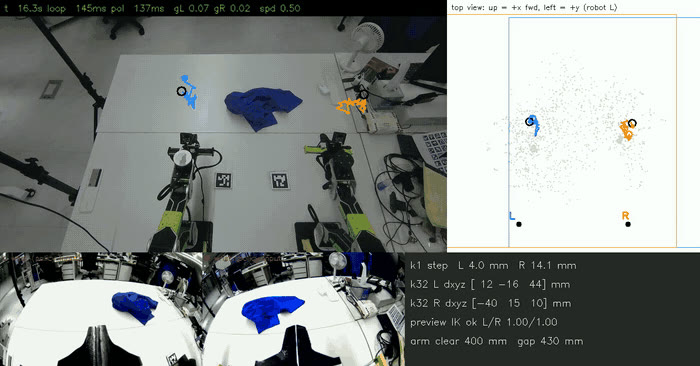
\includegraphics[width=\columnwidth]{figures/fig_deploy_ui.jpg}
\caption{Deploy UI in dry run (no command sent): predicted 32-step jaw-tip paths on the fixed camera (left blue, right
orange), top view in the robot base, both robot wrist cameras and the live checks.}
\label{fig:deploy}
\end{figure}
The policy runs in a receding-horizon loop (Fig.~\ref{fig:deploy}). Each cycle takes fresh images and the measured joints;
FK gives the current TCP; the policy predicts 32 relative steps; the newest TCP re-anchors the chunk to absorb latency; a
limiter bounds speed and the table floor; Pink IK solves the joints; and the safety checks of Sec.~\ref{sec:checks}
(workspace, link-to-link capsules, table, joint limits) must pass. Only the first 4 steps are committed before re-planning
(about 7\,Hz).

\textbf{Gripper safety.} On 27 October the bridge was restarted without the left-jaw opening limit, the left jaw opened to
the end of its travel and broke the holder. The deploy tool now refuses GO unless the bridge limits the left jaw to at most
half of its $-270^\circ$ travel. A jaw-only re-zero tool fixes a jaw whose zero has drifted (\code{robot_bridge/}).

\subsection{Decisions, 10-21 to 10-27}\label{sec:decisions}
\begin{table*}[t]
\caption{Decision log}\label{tab:decisions}
\centering\small
\begin{tabular}{@{}p{0.07\textwidth}p{0.44\textwidth}p{0.43\textwidth}@{}}
\toprule
date & finding & decision \\
\midrule
10-21 & The smooth old replay came from the data (tag gaps $\le$1.3\,s) plus a strong replay low-pass; executed vs tags was
28--35\mm & separate smoothness from accuracy; keep 0.25\,s smoothing on the label only \\
10-22 & Rig labels on the 10-22 takes were swapped against the wrist cameras & assign arms by table side, not by label \\
10-23 & Wrist-camera SLAM breaks at grasps; a gyro-bias check missed a 3.8$^\circ$/s bias (rotation 5--10$^\circ$ off) &
fixed-camera point tracking + tags become the pose source \\
10-24 & Tags fix the absolute error (42$\to$12\mm on a dev take); adding IMU acceleration made it worse & fusion variant
Cg: points + tags, IMU acceleration only inside gaps; strict hidden-tag hold-out \\
10-25 & 33 of 41 ``in view'' demos at the old camera height still had hands leaving the frame & raise the camera
(96$\to$105$\to$113\,cm) and re-record; no edge exits at 105/113\,cm \\
10-26 & IK$\to$FK labels bend the target at grasps (p95 $\approx$58\mm) & train on A; IK is a checker offline and the
executor online \\
10-26/27 & Still frames at the start and end; short tracking gaps at the edges & idle trim + edge-gap trim; fine-tune on
GOLD only \\
\bottomrule
\end{tabular}
\end{table*}
Table~\ref{tab:decisions} collects the decisions of this period with the finding behind each.

\subsection{Planned experiments}\label{sec:plannedexp}
No policy result is reported in this version. Two experiments are set up:
\begin{enumerate}
\item \emph{DiT, Soft-Fold pretrain $\to$ ours.} A diffusion transformer policy~\cite{peebles2023dit} with CLIP text
  conditioning~\cite{radford2021clip} (LeRobot \texttt{multi\_task\_dit}, 2 observation frames, horizon 33) is pretrained
  for 300k steps on the Soft-Fold bimanual folding data (1\,524 episodes, 2.1\,M frames at 20\,Hz) and fine-tuned on our
  GOLD demos for up to 300k steps. Checkpoints at 25k, 50k, 75k, 100k, 150k, 200k, 250k and 300k are compared on held-out
  error and grasp-phase metrics, not on training loss.
\item \emph{X-VLA, mixture pretrain $\to$ ours.} The X-VLA base model~\cite{xvla} is pretrained on a mix of Soft-Fold
  (domain 18), iPhUMI sweater folding~\cite{iphumi} (all 1\,572 episodes, domain 19) and PrimeBot UMI cloth
  episodes~\cite{primebot} (400 full episodes, domain 20), sampled 1\,:\,1\,:\,1 by training windows, then fine-tuned on our
  GOLD demos with a new domain 21 that starts untrained. The domain is asserted constant per episode. None of the public
  sets has a fixed global camera, so that input is blank for the UMI sets. A 1k-step smoke test on one RTX 5090 checks
  action scale, the 6-D rotation convention, left/right order, jaw polarity and camera order before the full run.
\end{enumerate}
Both are evaluated offline first (k16/k32 position and rotation error, split into grasp and free phases and early, middle
and late parts of the episode, against a zero-motion baseline), then on the robot by the operator.

% =====================================================================
\section{Discussion and Lessons}\label{sec:lessons}
\begin{enumerate}
\item \emph{Absolute tags plus depth beat SLAM for contact-rich hand motion.} The failure regime of SLAM (close range,
  textureless cloth, fast motion) is exactly the grasp.
\item \emph{Measure in the world, not in FK.} The 89\mm TCP error and the 70\mm base error were invisible to FK-based
  checks; tape, camera and real cloth found them.
\item \emph{Fix the conversion, do not add heuristics.} Lifting the jaws for finger-corner safety cost the grasp; allowing
  contact restored it.
\item \emph{One clock for everything.} It made camera, IMU and robot alignment, and the side-by-side videos, possible
  without sync hardware.
\item \emph{Model the controller.} The tracking error followed $\dot\tau_g/K_i$; changing $K_p$ could not help.
\item \emph{Grade the data instead of gating it.} Strict gates leave no usable egocentric data. Three data grades (replay /
  training / pretraining) and per-frame quality weights keep it usable. (v0.1: per-demo GOLD / SILVER / REJECT.)
\item \emph{Do not let the executor write the label} (v0.1). IK choices that are right for execution (roll relaxation,
  jaw flip) are wrong as training targets; the label stays Cartesian and the IK runs at execution time.
\item \emph{Anchor, do not replace} (v0.1). Point tracking covers the hidden phases, and the tags remove its absolute
  error; neither is enough alone.
\end{enumerate}

% =====================================================================
\section{Limitations and Threats to Validity}\label{sec:limits}
\begin{itemize}
\item \emph{No success rate.} Replays were judged by measurement and video; no trials were counted. One demo of one take
  was replayed in full on both arms, four times with the same plan; the 1\mm repeatability shows determinism, not
  generality across demos, demonstrators or garments.
\item \emph{What the parity metrics cannot see.} A, B and C are compared relative to the start of each window and C is
  shifted by its fitted lag, so constant offsets and delays do not count as error. C is the FK of the encoders and carries
  the same kinematic model as B. This is why the 89\mm TCP error passed every parity test. The absolute jaw position was
  checked only by tape at a few poses (Sec.~\ref{sec:rescal}) and by the Orbbec video.
\item \emph{Tag-hidden phases.} Position there is interpolated (21\% of the right-hand frames of demo~2) or taken from
  gated SLAM; its error is not measured at the grasps that matter most.
\item \emph{Jaw labels.} The classifier thresholds were tuned per hand by inspection; we have no held-out accuracy number
  on demo takes. The jaw leads were measured without load.
\item \emph{Table model.} The table is a plane at $z_\mathrm{t}=3$\mm in the right-arm base frame; the soft floor and
  clearances depend on it.
\item \emph{Video timing.} The Orbbec recording of run 200335 lost its timestamp file (the recorder was suspended), so its
  side-by-side video uses frame write times (about 10--30\,ms error).
\item \emph{Training data} (v0.1). The fusion accuracy is measured at hidden tags, which are mostly away from the grasp;
  the error inside long gaps is bounded only by the gates. The grades and the IK check above cover the first 139 demos; the
  remaining demos are processed with the same code. Success was judged by one person from one frame.
\end{itemize}

% =====================================================================
\section{Conclusion and Next Steps}\label{sec:next}
Replay of converted hand-worn-gripper demonstrations works as an end-to-end test: with one world frame and one clock, a
two-arm robot reproduces a full demonstration deterministically and brings its jaws to the human's grasp height, but it
does not yet fold like the human. The open problems and next steps are:
\begin{itemize}
\item \emph{Position error} of 17--30\mm RMSE over the demo against the replayed path (22--34\mm against the raw
  human path); the error at the grasp points themselves is not yet measured. Next, a per-grasp $xy$ error table from the
  videos: a constant bias points to calibration, a varying one to local visual correction at the grasp.
\item \emph{Open-loop replay needs the same scene.} Next, a cloth-placement reference before each replay.
\item \emph{Tag-hidden phases.} v0.1: addressed by point tracking + tags + IMU fusion with per-demo grades
  (Sec.~\ref{sec:trainpose}); MASt3R is no longer used.
\item \emph{Hardware.} The left wrist connector is intermittent, and the right arm has dropped power and USB.
\item \emph{Training.} v0.1: the 300-demo flattening set with Cartesian-before-IK labels is built; the two experiments
  of Sec.~\ref{sec:plannedexp} are next, then real-robot evaluation.
\end{itemize}

% =====================================================================
\appendices
\section{Running a session}\label{app:run}
\raggedright
\noindent\textbf{Interpreters.} \texttt{.venv} records and processes (Orbbec needs \texttt{sudo}); \texttt{xvla-mac}
plans and replays; the robot plugin's Python runs the bridge. Tool names are given without paths; options are shortened.

\noindent\textbf{Bring-up} (every session). Check the USB location IDs and gripper zeros;
\texttt{bridge\_start -{}-sides left,right -{}-go}; \texttt{ready\_pose -{}-side right|left -{}-go}.

\noindent\textbf{Calibration} (one-time, Sec.~\ref{sec:cal}).
\begin{itemize}
\item Camera$\leftrightarrow$robot: \texttt{robot\_cam\_poses -{}-side S -{}-go} (32 holds) $\to$
  \texttt{robot\_cam\_solve.py}.
\item Start markers: result in \code{configs/calibration/start_anchors_v001.json}.
\item Tag rig: \texttt{tag\_rig\_solve.py}, \texttt{tag\_rig\_pivot.py}.
\end{itemize}

\noindent\textbf{Data chain, in order} (Sec.~\ref{sec:conv}).
\begin{itemize}
\item $\to$D0 record: \texttt{sudo tag\_rig\_record -{}-proto task -{}-wrist} (start at markers 400/401).
\item D0$\to$D3 tags to jaw-tip trajectory: \texttt{umi\_tcp\_traj.py -{}-hand H -{}-depth -{}-imu-fill} for each hand
  (tag fusion: \texttt{tag\_rig\_fuse.py}); the IMU fill of D3$\to$D4 runs in the same call.
\item D3$\to$D4 optional SLAM (legacy, \code{legacy/scripts/mast3r_gapfill/}): \texttt{wrist\_m3\_prep.py} $\to$
  \texttt{run\_segmented.py} (GPU) $\to$ \texttt{umi\_slam\_eval.py -{}-save}.
\item D3$\to$D4 jaw state: \texttt{umi\_jaw infer} on \texttt{wrist/} and \texttt{wrist\_left/}.
\item D4$\to$D5 robotize: \texttt{umi\_robotize\_bi.py -{}-src \_fused -{}-clear 0 -{}-sep 0.06 -{}-min-reach 0}.
\item D5$\to$D6 + safety checks: \texttt{umi\_replay\_bi -{}-rep N -{}-traj \_fused\_robot -{}-speed 0.35 -{}-q-smooth 9
  -{}-max-ik-mm 15 -{}-tip-clear -0.01 -{}-tip-clear-left-extra 0 -{}-link-margin 0.015 -{}-max-rot-dev 25 -{}-offline}.
\item Plan$\to$D7 execute: the same with \texttt{-{}-go}, then \texttt{POST /rest}.
\item Compare D7: \texttt{replay\_parity.py}; \texttt{replay\_side\_by\_side.py [-{}-robot-time]}.
\end{itemize}

\noindent\textbf{Training-data chain} (v0.1, Sec.~\ref{sec:train}; stage numbers of Table~\ref{tab:stages}).
\begin{itemize}
\item 2: \texttt{umi\_jaw infer} (GPU) $\to$ \texttt{jaw\_aperture.py}.
\item 3--4: \texttt{umi\_tcp\_traj.py}; \texttt{robot\_cam\_from\_anchors.py} after a camera move; \texttt{new\_take\_prep.py},
  \texttt{tag\_rot\_extract\_v002.py}, \texttt{track\_v31.py}.
\item 5--6: \texttt{make\_pack2.py} $\to$ \texttt{run\_cotracker.py} (GPU) $\to$ \texttt{solve2.py} $\to$ \texttt{gate.py}.
\item 7--9: \texttt{trajectory\_fusion\_v1.py} (variant Cg) $\to$ \texttt{tighten\_trim.py}, \texttt{edge\_gap\_trim.py} $\to$
  \texttt{episode\_quality.py}, \texttt{render\_fusion\_qa.py}.
\item 10--12: \texttt{robotize\_ik.py} $\to$ \texttt{ik\_qa\_stats.py}; \texttt{tag\_rig\_unsplit.py -{}-label rob}
  (LeRobot); \texttt{tagrig\_offline\_eval.py}; \texttt{act\_tagrig\_deploy.py}.
\end{itemize}

\noindent\textbf{Safety.} The robot moves only with a person present. Plan offline before \texttt{-{}-go}. Park the arms
between tests; holding READY for hours overheated a motor. Stop the recorder with Ctrl+C, not Ctrl+Z, so that its
timestamps are saved. Start the bridge with the left-jaw opening limit; deploy refuses GO without it.

\section{Repository layout}\label{app:repo}
\begin{itemize}
\item \texttt{technical\_report/}: this report (LaTeX, figures, PDF).
\item \texttt{hardware/umihand/}: HandUMI build copy with our modifications, tag sheets and IMU firmware.
\item \texttt{visual\_teleop/}: recorder, jaw classifier, IK planner and replay, robot tools.
\item \texttt{scripts/}: calibration, tag pose, jaw aperture, robotization for replay, parity and side-by-side video.
\item \texttt{processing/}: the v0.1 training-data pipeline (point-tracking fusion, gates, trims, grades, labels, dataset,
  offline evaluation, deploy).
\item \texttt{robot\_bridge/}: reBot MIT bridge and gripper/joint zero tools.
\item \texttt{configs/}: calibration, robot settings and overrides, jaw weights.
\item \texttt{media/}: GIFs, videos and photos.
\item \texttt{legacy/}: earlier and dropped approaches (bare-hand collector, UMIalign smoother and exporter, red-tape jaw
  tools, Orbbec body tracking, Kalibr export, ORB-SLAM3 and stereo-VIO experiments; since v0.1 also the MASt3R gap filler
  \code{legacy/scripts/mast3r_gapfill/} and runner \code{legacy/slam/mast3r/}).
\end{itemize}
Raw takes, the robot plugin and the URDF are not included. ORB-SLAM3 (GPLv3) is represented only by our patch scripts.

\begin{thebibliography}{99}
\bibitem{chi2024umi} C.~Chi, Z.~Xu, C.~Pan, E.~Cousineau, B.~Burchfiel, S.~Feng, R.~Tedrake, and S.~Song, ``Universal
Manipulation Interface: In-the-wild robot teaching without in-the-wild robots,'' in \emph{Proc. Robotics: Science and Systems
(RSS)}, 2024. arXiv:2402.10329.
\bibitem{handumi} BrikHMP18 and murobotics-ai, ``HandUMI hardware (handumi-hw),'' GitHub repository, Apache-2.0, 2026.
\url{https://github.com/murobotics-ai/handumi-hw} (build copy from commit \texttt{e58de33}).
\bibitem{meza2026handumi} B.~Meza, L.~Perez, A.~Mendoza, A.~Ubillus, M.~Ramos, R.~Bastidas, M.~Olivera, and B.~Bastidas,
``HandUMI: A modular hand-worn parallel-jaw interface for robot-free bimanual data capture,'' 2026.
\url{https://murobotics.ai/research/handumi}
\bibitem{xu2025dexumi} M.~Xu, H.~Zhang, Y.~Hou, Z.~Xu, L.~Fan, M.~Veloso, and S.~Song, ``DexUMI: Using human hand as the
universal manipulation interface for dexterous manipulation,'' in \emph{Proc. Conf. Robot Learning (CoRL)}, PMLR vol.~305,
pp.~437--459, 2025. arXiv:2505.21864.
\bibitem{kareer2025egomimic} S.~Kareer, D.~Patel, R.~Punamiya, P.~Mathur, S.~Cheng, C.~Wang, J.~Hoffman, and D.~Xu,
``EgoMimic: Scaling imitation learning via egocentric video,'' in \emph{Proc. IEEE Int. Conf. Robotics and Automation
(ICRA)}, pp.~13226--13233, 2025. arXiv:2410.24221.
\bibitem{zhao2023aloha} T.~Z.~Zhao, V.~Kumar, S.~Levine, and C.~Finn, ``Learning fine-grained bimanual manipulation with
low-cost hardware,'' in \emph{Proc. Robotics: Science and Systems (RSS)}, 2023. arXiv:2304.13705.
\bibitem{cadene2024lerobot} R.~Cadene \emph{et al.}, ``LeRobot: State-of-the-art machine learning for real-world robotics in
PyTorch,'' 2024. \url{https://github.com/huggingface/lerobot}
\bibitem{avigal2022speedfolding} Y.~Avigal, L.~Berscheid, T.~Asfour, T.~Kr\"oger, and K.~Goldberg, ``SpeedFolding: Learning
efficient bimanual folding of garments,'' in \emph{Proc. IEEE/RSJ Int. Conf. Intelligent Robots and Systems (IROS)}, 2022.
arXiv:2208.10552.
\bibitem{ha2021flingbot} H.~Ha and S.~Song, ``FlingBot: The unreasonable effectiveness of dynamic manipulation for cloth
unfolding,'' in \emph{Proc. Conf. Robot Learning (CoRL)}, 2021. arXiv:2105.03655.
\bibitem{olson2011apriltag} E.~Olson, ``AprilTag: A robust and flexible visual fiducial system,'' in \emph{Proc. IEEE Int.
Conf. Robotics and Automation (ICRA)}, pp.~3400--3407, 2011.
\bibitem{wang2016apriltag2} J.~Wang and E.~Olson, ``AprilTag 2: Efficient and robust fiducial detection,'' in \emph{Proc.
IEEE/RSJ Int. Conf. Intelligent Robots and Systems (IROS)}, pp.~4193--4198, 2016.
\bibitem{bradski2000opencv} G.~Bradski, ``The OpenCV library,'' \emph{Dr.\ Dobb's Journal of Software Tools}, 2000.
\bibitem{collins2014ippe} T.~Collins and A.~Bartoli, ``Infinitesimal plane-based pose estimation,'' \emph{Int. J. Computer
Vision}, vol.~109, no.~3, pp.~252--286, 2014.
\bibitem{terzakis2020sqpnp} G.~Terzakis and M.~Lourakis, ``A consistently fast and globally optimal solution to the
perspective-n-point problem,'' in \emph{Proc. European Conf. Computer Vision (ECCV)}, pp.~478--494, 2020.
\bibitem{murai2025mast3rslam} R.~Murai, E.~Dexheimer, and A.~J.~Davison, ``MASt3R-SLAM: Real-time dense SLAM with 3D
reconstruction priors,'' in \emph{Proc. IEEE/CVF Conf. Computer Vision and Pattern Recognition (CVPR)}, 2025.
arXiv:2412.12392.
\bibitem{leroy2024mast3r} V.~Leroy, Y.~Cabon, and J.~Revaud, ``Grounding image matching in 3D with MASt3R,'' in
\emph{Proc. European Conf. Computer Vision (ECCV)}, 2024. arXiv:2406.09756.
\bibitem{wang2024dust3r} S.~Wang, V.~Leroy, Y.~Cabon, B.~Chidlovskii, and J.~Revaud, ``DUSt3R: Geometric 3D vision made
easy,'' in \emph{Proc. IEEE/CVF Conf. Computer Vision and Pattern Recognition (CVPR)}, 2024. arXiv:2312.14132.
\bibitem{campos2021orbslam3} C.~Campos, R.~Elvira, J.~J.~G\'omez~Rodr\'iguez, J.~M.~M.~Montiel, and J.~D.~Tard\'os,
``ORB-SLAM3: An accurate open-source library for visual, visual-inertial, and multimap SLAM,'' \emph{IEEE Trans. Robotics},
vol.~37, no.~6, pp.~1874--1890, 2021.
\bibitem{usenko2020basalt} V.~Usenko, N.~Demmel, D.~Schubert, J.~St\"uckler, and D.~Cremers, ``Visual-inertial mapping with
non-linear factor recovery,'' \emph{IEEE Robotics and Automation Letters}, vol.~5, no.~2, pp.~422--429, 2020.
\bibitem{geneva2020openvins} P.~Geneva, K.~Eckenhoff, W.~Lee, Y.~Yang, and G.~Huang, ``OpenVINS: A research platform for
visual-inertial estimation,'' in \emph{Proc. IEEE Int. Conf. Robotics and Automation (ICRA)}, pp.~4666--4672, 2020.
\bibitem{xu2025airslam} K.~Xu, Y.~Hao, S.~Yuan, C.~Wang, and L.~Xie, ``AirSLAM: An efficient and illumination-robust
point-line visual SLAM system,'' \emph{IEEE Trans. Robotics}, 2025 (accepted). arXiv:2408.03520.
\bibitem{furgale2013kalibr} P.~Furgale, J.~Rehder, and R.~Siegwart, ``Unified temporal and spatial calibration for
multi-sensor systems,'' in \emph{Proc. IEEE/RSJ Int. Conf. Intelligent Robots and Systems (IROS)}, pp.~1280--1286, 2013.
\bibitem{shah2013robotworld} M.~Shah, ``Solving the robot-world/hand-eye calibration problem using the Kronecker
product,'' \emph{J. Mechanisms and Robotics}, vol.~5, no.~3, 2013.
\bibitem{carpentier2019pinocchio} J.~Carpentier, G.~Saurel, G.~Buondonno, J.~Mirabel, F.~Lamiraux, O.~Stasse, and
N.~Mansard, ``The Pinocchio C++ library: A fast and flexible implementation of rigid body dynamics algorithms and their
analytical derivatives,'' in \emph{Proc. IEEE/SICE Int. Symp. System Integration (SII)}, 2019.
\bibitem{pink} S.~Caron \emph{et al.}, ``Pink: Python inverse kinematics based on Pinocchio,'' software, Apache-2.0.
\url{https://github.com/pink-kinematics/pink}
\bibitem{he2016resnet} K.~He, X.~Zhang, S.~Ren, and J.~Sun, ``Deep residual learning for image recognition,'' in
\emph{Proc. IEEE Conf. Computer Vision and Pattern Recognition (CVPR)}, 2016.
\bibitem{deng2009imagenet} J.~Deng, W.~Dong, R.~Socher, L.-J.~Li, K.~Li, and L.~Fei-Fei, ``ImageNet: A large-scale
hierarchical image database,'' in \emph{Proc. IEEE Conf. Computer Vision and Pattern Recognition (CVPR)}, pp.~248--255, 2009.
\bibitem{karaev2024cotracker3} N.~Karaev, I.~Makarov, J.~Wang, N.~Neverova, A.~Vedaldi, and C.~Rupprecht, ``CoTracker3:
Simpler and better point tracking by pseudo-labelling real videos,'' 2024. arXiv:2410.11831.
\bibitem{mahony2008ahrs} R.~Mahony, T.~Hamel, and J.-M.~Pflimlin, ``Nonlinear complementary filters on the special
orthogonal group,'' \emph{IEEE Trans. Automatic Control}, vol.~53, no.~5, pp.~1203--1218, 2008.
\bibitem{peebles2023dit} W.~Peebles and S.~Xie, ``Scalable diffusion models with transformers,'' in \emph{Proc. IEEE/CVF
Int. Conf. Computer Vision (ICCV)}, 2023.
\bibitem{radford2021clip} A.~Radford \emph{et al.}, ``Learning transferable visual models from natural language
supervision,'' in \emph{Proc. Int. Conf. Machine Learning (ICML)}, 2021.
\bibitem{xvla} X-VLA base model, \texttt{lerobot/xvla-base}, Hugging Face. \url{https://huggingface.co/lerobot/xvla-base}
\bibitem{iphumi} iPhUMI behavior-prompting data, \texttt{real-stanford/behavior\_prompting}, Hugging Face, MIT licence.
\bibitem{primebot} PrimeBot challenge data, \texttt{challenge-2026/challenge\_data}, Hugging Face, CC BY-SA 4.0.
\end{thebibliography}
\end{document}
